\documentclass[11pt]{article}

\usepackage[margin=1in]{geometry}
\usepackage{amsmath,amssymb}
\usepackage{graphicx}
\graphicspath{{./}{figs/}}
\usepackage{booktabs}
\usepackage{xcolor}
\usepackage{hyperref}
\hypersetup{colorlinks=true, linkcolor=blue, citecolor=blue, urlcolor=blue}
\usepackage{caption}
\usepackage{authblk}

\newcommand{\SBA}{S(B|A)}
\newcommand{\NMI}{\mathrm{NMI}}
\newcommand{\Strue}{S_{\rm true}}
\newcommand{\Itrue}{I_{\rm true}}

\title{Entropy and Mutual Information in Dijet Hadron Multiplicities:\\
Motivation, Interpretation Limits, and a Finite-Statistics Methodology}

\author[1,2]{Zhoudunming (Kong) Tu}
\affil[1]{Brookhaven National Laboratory}
\affil[2]{Stony Brook University}

\date{\today}

\begin{document}
\maketitle

\begin{abstract}
\noindent
The mutual information (MI) between the hadron multiplicities of
back-to-back jets is a new, information-theoretically complete measure
of inter-jet correlation, motivated by the entanglement-entropy
interpretation of hadron multiplicity distributions
\cite{KL2017,TKU2020,H1_2021,Datta2025}. We first establish precisely what
this observable can and cannot probe. Because hadron counting is a
single, fixed measurement, the joint multiplicity distribution is a
classical probability distribution, and its Shannon conditional entropy
and normalized MI obey $\SBA\geq0$ and $\NMI\leq1$ \emph{identically} --
these bounds cannot be violated by any dataset, whether or not the
underlying partonic state is entangled, so multiplicity-based entropies
cannot serve as a quantum witness. Their physics value lies elsewhere:
ansatz-conditional tests of the maximal-entanglement picture of
hadronization, an information-complete generalization of
forward--backward multiplicity correlations, discrimination between
hadronization models, and a quantitative classical-correlation baseline
for the broader quantum-information program at colliders. The core of
this note is the statistical problem of measuring these entropies
reliably at finite statistics. We show that the naive plug-in entropy/MI
estimator is systematically biased upward at finite event count~$N$, in
exactly the direction that mimics a genuine correlation excess. Using a
controlled Monte Carlo toy model with a known ground truth, we validate
two standard corrections (Miller--Madow and shuffle-subtraction) and a
more rigorous Bayesian estimator (NSB, Nemenman--Shafee--Bialek). We then
validate the full pipeline -- cross-checked between independent Python
and ROOT/C++ implementations -- on realistic PYTHIA~8 dijet Monte Carlo,
introduce the scale-comparable normalized observable
$\NMI=I(A{:}B)/\min(S_A,S_B)$, and document a genuine
bootstrap-consistency pitfall uncovered during cross-validation together
with its fix. Finally, since PYTHIA~8 output has no independently known
true MI, we develop a Tier-2 closure test that calibrates a synthetic
model to the real data's own statistics to obtain a trustworthy
pseudo-truth. Applied to the whole validation sample, this shows NSB's
bootstrap uncertainty under-covers by a factor of roughly $1.5$--$1.7$;
applied differentially in leading-jet-$p_T$ bins, with a separate
calibrated model fit per bin, the same test finds substantially
better-calibrated (though still imperfect) coverage, suggesting the
whole-sample under-coverage is at least partly an artifact of fitting one
model across a range of $p_T$-dependent structure. Both results are
reported as quantitative calibration factors to be applied explicitly
before quoting any uncertainty on real detector data, not as corrections
silently folded into the pipeline.
\end{abstract}

\tableofcontents

% =============================================================================
\section{Physics motivation and what this observable can teach}
\label{sec:motivation}
% =============================================================================

Take a back-to-back dijet event (e.g.\ from $e^+e^-$, DIS, or $pp$
collisions at RHIC/STAR). Treat jet $A$ and jet $B$ as the two subsystems
of a bipartite system whose ``state'' is accessed only through observed
hadron multiplicities, via \textbf{local parton--hadron duality (LPHD)}:
the hadron multiplicity distribution stands in for the underlying parton
Fock-state distribution.

\textbf{The Schmidt-decomposition ansatz}
\cite{KL2017,PS2016}: if each Fock/parton-number sector $n$ carries
probability $P(n)$, and the reduced density matrix of a jet is diagonal in
$n$, then the entanglement entropy of that jet reduces to the
\textbf{Shannon entropy of its hadron multiplicity distribution},
\begin{equation}
S_A = -\sum_n P_A(n)\ln P_A(n),
\end{equation}
and likewise for $S_B$. This identification underlies the successful
comparison of measured hadron entropies with entanglement-entropy
predictions in DIS \cite{TKU2020,H1_2021} and, recently, in jet
fragmentation \cite{Datta2025}.

\textbf{The measurement proposed here:} by additionally recording the
\emph{joint} multiplicity distribution $P_{AB}(n_A,n_B)$ across both jets
in the same event, one can construct the mutual information $I(A{:}B)$,
the conditional entropy $\SBA$, and a normalized mutual information
$\NMI$ (all defined in Sec.~\ref{sec:observable}) -- extending the
single-jet entropy program to the two-jet, correlation level.

\textbf{An interpretation limit, stated up front.} As shown in detail in
Sec.~\ref{sec:nogo}, these multiplicity-based entropies \emph{cannot} be
used to witness or certify quantum correlations: the measured joint
distribution is, by construction, a classical probability distribution,
for which $\SBA\geq0$ and $\NMI\leq1$ hold as mathematical identities --
no data, however entangled its partonic origin, can violate them. The
motivation for the measurement is therefore \emph{not} a
classical-bound-violation test. (Sec.~\ref{sec:qmodel} shows how models
with genuine quantum correlations are nonetheless confronted with the
data: by projecting the model down to the measured number-basis
statistics, never by lifting the data up to the state.) What the
observable genuinely teaches is the following.

\begin{enumerate}

\item \textbf{Ansatz-conditional tests of the entanglement picture of
hadronization.} Under the Schmidt/LPHD ansatz, a \emph{pure} bipartite
dijet state predicts equal von Neumann marginal entropies, hence
(via the ansatz) the testable relation $S_A \simeq S_B$ even for
kinematically asymmetric jet selections; and in the idealized Schmidt
limit the two multiplicities are perfectly correlated, $\NMI\to1$. Where
the measured $\NMI$ sits between the independent limit ($\NMI=0$) and the
Schmidt limit ($\NMI=1$) quantifies how much of the initial state's
correlation structure survives hadronization as classical correlation --
extending the single-jet entropy tests of
Refs.~\cite{TKU2020,H1_2021,Datta2025} to the joint two-jet level.

\item \textbf{An information-complete generalization of
forward--backward multiplicity correlations.} The classic
forward--backward correlation strength $b_{\rm corr}$
\cite{ALICE2015fb} is a linear (second-moment) statistic. $I(A{:}B)$
captures \emph{all} statistical dependence between the two multiplicities
at once -- every moment, including nonlinear structure -- and $\NMI$
makes the result dimensionless and comparable across collision energies,
kinematic selections, and experiments. No dijet multiplicity MI
measurement exists to date; it is a new correlation observable even as
pure QCD.

\item \textbf{Hadronization-model discrimination.} String and cluster
hadronization predict different cross-jet correlation topologies -- in
$e^+e^-$ dijets a single string spans both hemispheres, so string
dynamics predicts specific long-range hemisphere multiplicity
correlations that cluster models do not share. Differential MI vs.\ jet
$p_T$ and cone radius $R$ is a tuning-grade generator constraint that
$b_{\rm corr}$ alone does not provide.

\item \textbf{Separation of classical correlation sources.} In $pp$
collisions, cross-jet correlations mix conservation laws
(energy--momentum, charge, strangeness -- calculable), color coherence
(concentrated at small $R$), initial-state fluctuations, and
multi-parton interactions / underlying event (scaling with event
activity). MI measured differentially in $p_T$, $R$, and event activity
decomposes these contributions.

\item \textbf{Sensitivity to (though not certification of) quantum
dynamics.} Quantum interference alters the \emph{diagonal}
$P_{AB}(n_A,n_B)$ even after the coherences are lost: coherent vs.\
independent gluon emission, Bose enhancement, and color reconnection all
leave imprints in the joint multiplicity distribution. A measured MI in
excess of classical-cascade generator baselines would be evidence of
dynamics those generators lack -- a discovery-grade anomaly, even though
not a nonclassicality certificate (Sec.~\ref{sec:nogo}).

\item \textbf{A rigorous classical-correlation envelope.} For any
underlying quantum state, the number-basis Shannon MI measured here is a
lower bound on the classical-correlation content $J(A{:}B)$ of that
state. It is therefore a required input to any future decomposition of
total vs.\ classical correlations using other degrees of freedom (e.g.\
spin), a program outside the scope of this note.

\item \textbf{Extensions to nuclear environments.} Dijet multiplicity MI
in $AA$ relative to $pp$ measures medium-induced decorrelation of the jet
pair -- an entropy-language counterpart of jet quenching -- and at the
EIC, current-jet vs.\ target-fragmentation entropy correlations probe the
$x$-dependence of the initial state's entanglement structure, the
original context of Ref.~\cite{KL2017}.

\end{enumerate}

\textbf{Why this is subtle in practice:} every one of the measurements
above requires entropies of a two-dimensional multiplicity histogram
estimated from a finite event sample, and MI estimated from a finite
sample is \textbf{always statistically biased} -- as shown below, biased
in exactly the direction that mimics a genuine correlation excess if not
handled carefully. The central technical content of this note is
therefore statistical: establishing, with controlled ground truth and
realistic generator validation, which estimators can be trusted, at what
sample sizes, with what calibrated uncertainties.

% =============================================================================
\section{The observables, their classical bounds, and why they cannot
witness quantum correlations}
\label{sec:observable}
% =============================================================================

From the per-jet and joint hadron-multiplicity distributions we can build
three entropies and two derived quantities:
\begin{equation}
S_A,\quad S_B,\quad S_{AB}
\qquad\Longrightarrow\qquad
I(A{:}B) = S_A+S_B-S_{AB},
\qquad
\SBA = S_{AB}-S_A .
\end{equation}

\paragraph{Elementary bounds.} For \emph{any} joint probability
distribution, two classical inequalities hold \cite{CoverThomas}:
\emph{subadditivity}, $S_{AB}\leq S_A+S_B$, equivalent to $I(A{:}B)\geq0$;
and \emph{monotonicity}, $S_{AB}\geq\max(S_A,S_B)$ (``conditioning cannot
make entropy negative''), equivalent to
\begin{equation}
\SBA \geq 0, \qquad S(A|B)\geq 0,
\qquad\Longleftrightarrow\qquad
I(A{:}B)\leq\min(S_A,S_B).
\label{eq:monotonicity}
\end{equation}
The one-line proof of monotonicity: $\SBA=\sum_a p(a)\,S(B|A{=}a)$ is a
convex combination of ordinary entropies, each of which is non-negative.
(We are careful to call Eq.~\eqref{eq:monotonicity} monotonicity rather
than subadditivity: the distinction matters below, because quantum von
Neumann entropy \emph{obeys} subadditivity but \emph{violates}
monotonicity for entangled states \cite{CerfAdami}.)

\paragraph{A scale-comparable form: normalized mutual information.}
Absolute $I(A{:}B)$ is awkward to compare across different collision
energies, kinematic selections, or $p_T$ bins, since $S_A$ and $S_B$
themselves grow with e.g.\ jet $p_T$ (Sec.~\ref{sec:pythia-ptdep}) and so
set a different natural scale for $I$ in every bin. The
$\min(S_A,S_B)$ appearing in Eq.~\eqref{eq:monotonicity} already does the
needed normalization:
\begin{equation}
\NMI \;\equiv\; \frac{I(A{:}B)}{\min(S_A,S_B)} \, .
\end{equation}
By monotonicity, $\NMI\in[0,1]$ for any distribution: $\NMI=0$ is the
independent limit and $\NMI=1$ is perfect correlation -- the Schmidt
limit of the entanglement ansatz (Sec.~\ref{sec:motivation}). Since
$\NMI$ is dimensionless and bounded, it is directly comparable across
$p_T$ bins, run periods, or even experiments in a way raw $I(A{:}B)$ is
not. This is a standard normalization in the wider MI literature (one of
several conventional choices, e.g.\ Kv\aa{}lseth \cite{Kvalseth1987};
$\min$-normalization is the tightest of these).

% -----------------------------------------------------------------------------
\subsection{Why no multiplicity measurement can violate these bounds}
\label{sec:nogo}
% -----------------------------------------------------------------------------

It is tempting to hope that, since the quantum (von Neumann) conditional
entropy of an entangled state can be negative \cite{CerfAdami}, a
sufficiently precise measurement of $\SBA$ from multiplicities could
reveal $\SBA<0$ (equivalently $\NMI>1$) and thereby certify a quantum
signature. This hope fails -- not for practical reasons, but in
principle. The argument has four steps, in increasing order of physical
content.

\paragraph{(i) The bounds are properties of distributions, not of
physics.} Any dataset of event-by-event pairs $(n_A,n_B)$ defines a joint
probability distribution -- the histogram itself. Monotonicity,
Eq.~\eqref{eq:monotonicity}, holds for \emph{every} joint probability
distribution, with no assumption about the dynamics that generated it.
There is therefore no possible measured $P_{AB}$ -- from PYTHIA, from
STAR data, or from the decay of a maximally entangled partonic state --
whose population-level $\SBA$ is negative or whose $\NMI$ exceeds one.
The bound is arithmetic, not a null hypothesis.

\paragraph{(ii) Where quantum negativity lives, and why counting cannot
reach it.} Negative conditional entropy is a property of the von Neumann
entropies of the quantum state $\rho_{AB}$ \emph{before} measurement.
Writing $\rho_{AB}$ in the number basis, the recorded counts determine
exactly the diagonal matrix elements,
$\langle n_A,n_B|\rho_{AB}|n_A,n_B\rangle = P_{AB}(n_A,n_B)$, and
nothing else: every off-diagonal element (coherence between different
multiplicity sectors) drops out of the counting statistics identically,
for any number of events. But the von Neumann entropy is a function of
the \emph{eigenvalues} of the full matrix, and the eigenvalues depend on
the coherences. A minimal example makes the information loss exact: the
entangled pure state
$|\psi\rangle=\sum_n\sqrt{\lambda_n}\,|n\rangle_A|n\rangle_B$ (with
$S(\rho_{AB})=0$) and the classical mixture
$\rho=\sum_n\lambda_n|n,n\rangle\langle n,n|$ (with
$S(\rho_{AB})=-\sum_n\lambda_n\ln\lambda_n>0$) produce \emph{identical}
joint counts, $P_{AB}(n_A,n_B)=\lambda_{n_A}\delta_{n_An_B}$, event
after event. Two states whose joint entropies differ by several nats
generate exactly the same dataset, so $S(\rho_{AB})$ is simply not a
function of the data recorded. Measuring $N_A$ and $N_B$
\emph{simultaneously} does not help: the two are a \emph{commuting}
pair -- a single measurement setting -- just as measuring $\sigma_z$ on
arbitrarily many copies of a qubit pins down
$\langle\sigma_z\rangle$ perfectly while leaving
$\langle\sigma_x\rangle$, $\langle\sigma_y\rangle$, and hence the state
and its entropy, undetermined. More fundamentally, entropy is not an
observable in the quantum-mechanical sense: it is nonlinear in $\rho$,
so no Hermitian operator has $S(\rho)$ as its expectation value. Every
laboratory determination of an entropy proceeds either through full
state tomography (requiring measurements in non-commuting bases) or
through collective measurements on multiple copies (e.g.\ a swap test
yielding $\mathrm{Tr}\,\rho^2$, which requires coherently interfering
two events with each other -- something no detector does; a large event
sample is many separate destructive measurements, not one joint coherent
one). Equivalently, in entropy language: measurement in the number basis
dephases $\rho_{AB}$ to its diagonal, and dephasing never decreases
entropy, so the Shannon $S_{AB}$ of the counts is an \emph{upper bound}
on the von Neumann $S(\rho_{AB})$, with the gap being exactly the
coherence content -- the excess entropy added by dephasing destroys
precisely the negativity one hoped to observe.

\paragraph{(iii) No complementary basis exists for multiplicity.} One
might try to repair (ii) by measuring in a second, non-commuting basis --
the strategy underlying every Bell-type test. For hadron multiplicity no
such basis exists, even in principle. Final-state hadron number is a
superselected, classically recorded quantity: no detector observable
connects different-multiplicity sectors coherently. More broadly,
\emph{every} function of the final-state hadron momenta -- multiplicity,
$p_T$-weighted multiplicity, jet shapes, substructure observables,
alternative cone radii -- commutes with every other such function, since
all are functions of the same recorded phase-space configuration.
Enlarging the set of jet observables therefore only enlarges one
classical joint distribution; it never supplies the basis rotation a
witness requires. Certifying nonclassical correlations at a collider
requires a degree of freedom with an analyzable post-hoc basis choice --
for example hadron spin accessed through self-analyzing weak decays
\cite{GPTV2022,AfikDeNova2023} -- which is a separate program, outside
the scope of this note.

\paragraph{(iv) The estimator-level corollary.} The plug-in estimate
obeys $\widehat{\SBA}\geq0$ \emph{exactly}, for every finite dataset,
because the empirical distribution is itself a probability distribution
to which Eq.~\eqref{eq:monotonicity} applies. Only bias-corrected
estimators (Miller--Madow, NSB; Secs.~\ref{sec:corrections}--\ref{sec:nsb})
can return $\widehat{\SBA}<0$ or $\widehat{\NMI}>1$, and only through
estimation error. Any apparently significant violation of the classical
bounds in an analysis is therefore \emph{guaranteed} to be a
finite-sample artifact, and must shrink as $N$ grows. This reframes the
statistical task of this note: the estimator machinery below is not
protecting a potential discovery claim from false positives -- it ensures
that the measured classical correlation quantities are unbiased and carry
honest uncertainties, and that boundary-hugging artifacts
($\widehat{\SBA}$ near or below zero, $\widehat{\NMI}$ near or above one)
are recognized as estimator pathology rather than physics.

% -----------------------------------------------------------------------------
\subsection{What the entanglement ansatz does and does not license}
% -----------------------------------------------------------------------------

The identification of the marginal Shannon entropy $S_A$ with an
entanglement entropy is a \emph{model statement}: it requires the
Schmidt/LPHD assumptions (a near-pure bipartite state whose reduced
density matrices are diagonal in the number sectors). Under those
assumptions the measurement acquires interpretive power: $S_A\simeq S_B$
tests the purity prediction; the measured entropies can be compared
against entanglement-entropy predictions computed from parton
distributions or fragmentation functions \cite{KL2017,TKU2020,H1_2021,
Datta2025}; and the position of $\NMI$ within $[0,1]$ measures how close
the jet pair sits to the Schmidt (perfectly correlated) limit. These are
consistency tests of an entanglement-based model against alternatives --
legitimate and falsifiable -- but consistency cannot be promoted to
certification: a classical mechanism producing the same joint
distribution is never excluded by this observable alone
(Sec.~\ref{sec:nogo}).

\paragraph{Quantum discord is likewise out of reach.} True
(Ollivier--Zurek \cite{OZ2001}) quantum discord is defined by optimizing
conditional entropy over quantum measurement bases -- non-commuting
projective measurements that do not reduce to reading off a classical
value. For any classical joint distribution -- and by (ii) above,
hadron-multiplicity data is one -- the optimal ``measurement'' on $B$ is
trivially observing $N_B$ exactly, which makes the classical-correlation
piece $J(A{:}B)$ equal to the \emph{full} $I(A{:}B)$, so discord
$D=I-J\equiv0$ identically, with no exception. Extracting a genuinely
nonzero discord requires actual quantum-state tomography of a different
degree of freedom \cite{AfikDeNova2023,GPTV2022}, not multiplicity
counting. What the multiplicity measurement contributes to that broader
program is the classical-correlation envelope of
Sec.~\ref{sec:motivation}, item~6 -- the rest of this note is about
measuring it reliably.

% -----------------------------------------------------------------------------
\subsection{Comparing to models with quantum correlations}
\label{sec:qmodel}
% -----------------------------------------------------------------------------

The no-go of Sec.~\ref{sec:nogo} does not prevent confronting the data
with a model in which the dijet system is genuinely entangled; it only
fixes the \emph{direction} of the comparison. The data can never be
lifted up to $S(\rho_{AB})$, but a quantum model can always be projected
down to the data: by the Born rule, the model predicts the outcome
statistics of the measurement actually performed. The comparison
therefore happens at the Shannon level, where the data lives, with the
model's von Neumann quantities acting as internal parameters whose
\emph{fingerprints} on the number-basis diagonal are what is tested.

The construction has three layers.

\begin{enumerate}
\item \textbf{The state.} Take the entanglement-based model of the dijet
in Schmidt form,
\begin{equation}
|\psi\rangle=\sum_n \sqrt{\lambda_n}\,|n\rangle_A\,|n\rangle_B,
\end{equation}
with the Schmidt weights $\lambda_n$ supplied by QCD -- from small-$x$
evolution / $xG(x,Q^2)$ in the Kharzeev--Levin picture \cite{KL2017}, or
from fragmentation functions as in Ref.~\cite{Datta2025}. The model's
quantum-information content is explicit and computable:
$S(\rho_{AB})=0$ (purity),
$S(\rho_A)=S(\rho_B)=-\sum_n\lambda_n\ln\lambda_n$ (the entanglement
entropy), and a negative quantum conditional entropy,
$S(B|A)_{\rm vN}=-S(\rho_A)<0$. None of this is directly measurable --
it is the model's internal bookkeeping.
\item \textbf{Dephasing (the measurement).} The predicted parton-level
joint distribution is the number-basis diagonal,
$P(n,m)=\lambda_n\delta_{nm}$. Note what happens to each quantum
quantity under this projection. The marginal entropy survives intact:
$\rho_A$ is diagonal in $n$, so its von Neumann entropy \emph{equals}
the Shannon entropy of the marginal counts -- this is exactly what the
Schmidt/LPHD ansatz buys, and why the single-jet entropy program
\cite{TKU2020,H1_2021,Datta2025} is well posed. The joint purity does
\emph{not} survive: the Shannon entropy of the diagonal is $S_A$, not
zero. The unobservable negativity is replaced by its measurable shadow,
\textbf{perfect correlation}: $\SBA=0$ and $\NMI=1$ at parton level.
\item \textbf{Hadronization as a channel.} Hadrons are not partons, so
each jet's multiplicity is smeared by a local transfer kernel,
$T(N_A|n)$ and $T'(N_B|n)$ (LPHD in its sharpest form is the identity
kernel; more realistically a Poisson- or NBD-like smearing around $n$).
The full prediction is
\begin{equation}
P_{AB}(N_A,N_B)=\sum_n \lambda_n\,T(N_A|n)\,T'(N_B|n).
\label{eq:schmidt-channel}
\end{equation}
From Eq.~\eqref{eq:schmidt-channel} the model's $S_A$, $S_B$,
$I(A{:}B)$, $\NMI$, and $\SBA$ follow -- all Shannon quantities,
directly comparable to the measured ones with the estimator and
calibration machinery of the rest of this note.
\end{enumerate}

\paragraph{Where the quantum content shows up in measurables.} The
model's quantumness translates into three concrete, falsifiable
predictions on the diagonal: purity of the state predicts
$S_A\simeq S_B$ even for kinematically asymmetric selections; the
entanglement-entropy identification predicts the \emph{value} of $S_A$
from $xG$ or the fragmentation functions; and the Schmidt structure
predicts $\NMI$ near its maximum, degraded from $1$ only by the
calculable smearing of the $T$ kernels -- whereas classical cascade
baselines sit at $\NMI\ll1$ (Sec.~\ref{sec:pythia}) with no reason to
approach the ceiling. The measurement therefore discriminates the
entanglement-structured prediction from generator baselines
quantitatively. It is a genuine model comparison -- it is just not a
certification.

\paragraph{The honest limit: the degeneracy class.}
Equation~\eqref{eq:schmidt-channel} depends on $\rho_{AB}$ only through
its diagonal. The pure state $|\psi\rangle$ and its fully dephased
classical twin, $\rho=\sum_n\lambda_n|n,n\rangle\langle n,n|$ -- with
$S(\rho_{AB})=0$ and $-\sum_n\lambda_n\ln\lambda_n$, respectively --
predict \emph{identical} data. The measurement thus constrains the
\emph{diagonal equivalence class} of states; within that class, the
value of $S(\rho_{AB})$ is a theoretical commitment, not an observable.
This is the no-go of Sec.~\ref{sec:nogo} seen from the model side, and
it should be stated in any comparison: ``the data agree with the
entanglement-based prediction'' and ``the data agree with its dephased
classical twin'' are the same sentence. Distinguishing members of the
class requires access to the coherences -- a different degree of
freedom, e.g.\ spin \cite{GPTV2022,AfikDeNova2023}, outside the scope of
this note.

\paragraph{Connection to the toy model.}
Equation~\eqref{eq:schmidt-channel} is a latent variable (the Schmidt
index $n$, drawn from $\lambda_n$) feeding two conditionally independent
emission kernels. This is structurally identical to the Gamma-Poisson
toy model of Sec.~\ref{sec:toymc}: the latent $\Lambda$ plays the role
of a continuous Schmidt spectrum, and the Poissons play the role of $T$.
The toy model used throughout this note is, in other words, the dephased
image of a Schmidt-form state -- so the estimator, bias, and closure
machinery developed below applies to quantum-model predictions without
modification, and the eventual data comparison reduces to a sharp,
well-posed question: which latent spectrum and kernels does nature use
-- those predicted by QCD entanglement ($\lambda_n$ from $xG$ or
fragmentation functions), or those produced by a classical cascade?

% =============================================================================
\section{The statistical problem: finite-sample bias}
\label{sec:bias}
% =============================================================================

Every quantity above is estimated from a finite event sample, and the
naive (``plug-in'') entropy estimator has a \textbf{systematic, structural
bias} that turns out to point in exactly the dangerous direction for this
measurement.

\paragraph{Where the bias comes from.} The naive estimator replaces true
probabilities $p_i$ with empirical frequencies $\hat p_i=n_i/N$,
\begin{equation}
\hat S = -\sum_i \hat p_i \ln \hat p_i .
\end{equation}
Because $x\ln x$ is convex (equivalently $-x\ln x$ is concave), Jensen's
inequality guarantees
\begin{equation}
\langle \hat S \rangle \;<\; \Strue \qquad \text{for any finite } N,
\end{equation}
i.e.\ the plug-in estimator always underestimates entropy. This isn't a
numerical artifact; with only $N$ draws one can never fully resolve a
distribution's tails, and that missing resolution always looks like
\emph{less} apparent randomness than there truly is.

\paragraph{Leading-order size of the effect} (Miller 1955
\cite{Miller1955}), for a distribution over $K$ possible outcomes:
\begin{equation}
\langle \hat S \rangle \approx \Strue - \frac{K-1}{2N}.
\end{equation}
Fewer events ($N$ small) or finer binning ($K$ large) both make the
downward bias worse.

\paragraph{Why this flips sign and biases $I(A{:}B)$ upward.} Combining
the individual biases of $\hat S_A,\hat S_B,\hat S_{AB}$ with correct
signs,
\begin{equation}
\langle\hat I\rangle \;\approx\; \Itrue +
\frac{(K_{AB}-1)-(K_A-1)-(K_B-1)}{2N}
= \Itrue + \frac{K_{AB}-K_A-K_B+1}{2N}.
\label{eq:mi-bias}
\end{equation}
The joint distribution lives in a much larger space than either marginal
alone, so $\hat S_{AB}$ suffers a \emph{much larger} downward bias than
$\hat S_A+\hat S_B$ does -- and since $S_{AB}$ enters with a
\textbf{minus} sign, its extra negative bias flips into a \textbf{positive}
bias on $\hat I$. In the extreme case $N \ll K_A K_B$ (badly undersampled
joint histogram), this produces large \emph{phantom} apparent mutual
information even for truly independent variables -- sampling noise alone
can masquerade as a real correlation excess. By the same mechanism it
pushes $\widehat{\SBA}$ spuriously downward toward -- and, for
bias-corrected estimators, even past -- the classical boundary that
Sec.~\ref{sec:nogo} showed the true quantity can never cross: finite
statistics manufactures exactly the boundary-hugging artifacts that make
uncorrected entropy measurements untrustworthy.

A commonly-quoted shortcut version of Eq.~\eqref{eq:mi-bias} is
$(K_A-1)(K_B-1)/(2N)$; this is not a different formula, it is
Eq.~\eqref{eq:mi-bias} evaluated under the extra assumption
$K_{AB}=K_AK_B$, i.e.\ a fully and uniformly occupied joint space. That
assumption only holds for independent variables; for correlated data the
observed $K_{AB}$ is much smaller than $K_AK_B$ (the joint distribution
concentrates on a narrow ridge rather than filling the full grid), so this
shortcut badly \emph{overestimates} the bias -- a pitfall we hit directly
in Sec.~\ref{sec:corrections}.

\paragraph{Practical consequence.} Comparing the same underlying physics
across data samples of different size -- different STAR running periods,
different luminosity, different jet-cone or multiplicity binning choices
-- will report systematically different central MI (and $\SBA$) values
purely from this effect, with zero change in the actual QCD physics.
Secs.~\ref{sec:toymc}--\ref{sec:nsb} demonstrate this concretely with a
toy model and work through three ways to correct for it;
Secs.~\ref{sec:pythia}--\ref{sec:closure} then validate the corrected
pipeline on realistic generator output and calibrate its uncertainties.

% =============================================================================
\section{Toy Monte Carlo test bed}
\label{sec:toymc}
% =============================================================================

To demonstrate the bias concretely and validate corrections against a
known ground truth, we use a controlled toy model: two back-to-back jets,
$A$ and $B$, with a shared latent hard-process fluctuation $\Lambda$
(e.g.\ fluctuating parton virtuality / initial-state energy scale) drawn
from a Gamma distribution. Conditional on $\Lambda$, each jet's hadron
multiplicity is Poisson distributed,
\begin{equation}
\Lambda \sim \mathrm{Gamma}(k,\theta), \qquad
N_A\,|\,\Lambda \sim \mathrm{Poisson}(\Lambda), \qquad
N_B\,|\,\Lambda \sim \mathrm{Poisson}(c\,\Lambda).
\end{equation}
Marginalizing over $\Lambda$ gives each jet a \textbf{Negative Binomial}
multiplicity distribution (the standard KNO-like form used for hadron
multiplicities), and the shared $\Lambda$ induces a genuine -- but purely
\textbf{classical} -- correlation between $N_A$ and $N_B$, i.e.\
$\Itrue>0$ with $\SBA_{\rm true}$ solidly positive. This is a convenient
sandbox: we know the true joint distribution (to arbitrary precision,
from a huge reference sample), so we can measure the \emph{bias} of any
estimator directly. Parameters used throughout: $k=3.0$, $\theta=8.0$,
$c=0.9$ (giving $\mathrm{corr}(N_A,N_B)\approx 0.88$). As noted in
Sec.~\ref{sec:qmodel}, this shared-latent structure is also exactly the
dephased image of a Schmidt-form entangled state, with $\Lambda$ playing
the role of a continuous Schmidt spectrum -- the machinery validated
here therefore applies unchanged to the predictions of
entanglement-based models.

\subsection{Demonstration: two samples, same true distribution, different
size}

We generate a ``small'' event sample ($N=500$; e.g.\ a single limited run
/ low-luminosity STAR-like dataset), a ``large'' event sample
($N=200{,}000$; high-statistics dataset), and a very large reference
sample ($N=5\times10^6$) to pin down $\Itrue$ -- all drawn from the
\emph{exact same underlying physics}.\footnote{The toy-model tables in
this and the following sections (Tables~\ref{tab:three-samples},
\ref{tab:corrections}, and \ref{tab:all-estimators}) were each generated
from independent random draws; entries at the same nominal $N$ therefore
differ between tables by ordinary sampling scatter. That scatter is
itself a preview of the estimator variance quantified in
Secs.~\ref{sec:corrections}--\ref{sec:nsb}.}

\begin{table}[h]
\centering
\caption{Naive $\hat I$ for three samples of the same true physics.}
\label{tab:three-samples}
\begin{tabular}{lrrrrr}
\toprule
Sample & $N$ & $K_A$ & $K_B$ & $K_{AB}$ & $\hat I_{\rm naive}$ (nats) \\
\midrule
small & 500 & 67 & 60 & 390 & 1.7424 \\
large & 200{,}000 & 129 & 113 & 3949 & 0.7463 \\
reference & 5{,}000{,}000 & 159 & 147 & 7022 & 0.7329 $\;(\approx \Itrue)$ \\
\bottomrule
\end{tabular}
\end{table}

We see $\hat I_{\rm small} > \hat I_{\rm large} \approx \hat I_{\rm ref}
\equiv \Itrue$ -- \textbf{the same physics, analyzed with fewer events,
reports a systematically larger MI}. This is the bias predicted in
Sec.~\ref{sec:bias}, not a change in physics.

The bias comes entirely from how well-populated the joint histogram is.
Figure~\ref{fig:marginals-joint} shows (top) the marginal
hadron-multiplicity distributions $P_A(n)$, overlaid for the three
samples -- these look reasonably similar even at $N=500$ because there are
only $O(10^2)$ bins to fill -- and (bottom) the 2D joint histograms
$P_{AB}(n_A,n_B)$ on the same color scale, where the difference is
dramatic: at $N=500$ the joint plane is almost empty, while at
$N=5\times10^6$ it is a smooth, fully-resolved correlated ridge. A sparse,
``salt-and-pepper'' joint histogram is exactly what drives $\hat S_{AB}$
artificially low, and hence $\hat I$ artificially high.

\begin{figure}[htb]
\centering
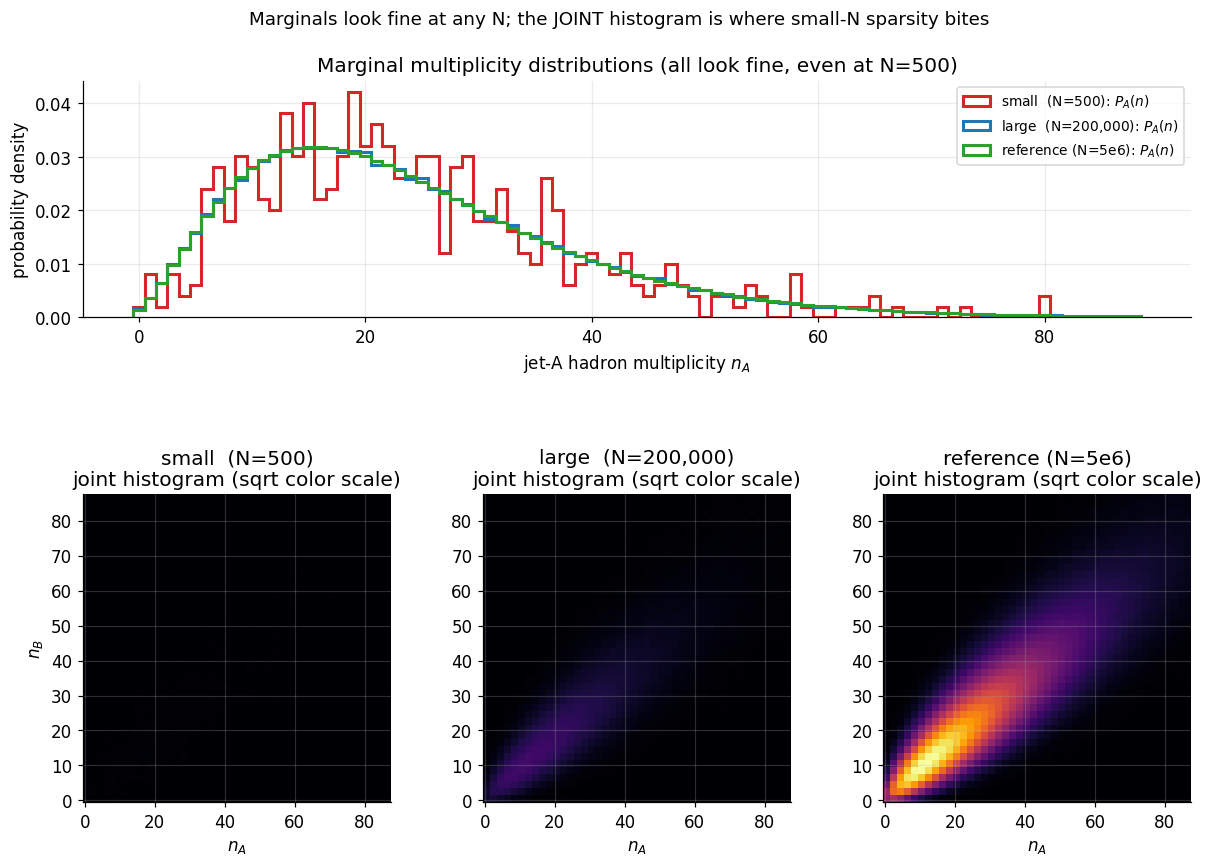
\includegraphics[width=\textwidth]{figs/fig01_marginals_joint.png}
\caption{Marginal multiplicity distributions (top) and 2D joint histograms
(bottom, square-root color scale) for the small, large, and reference
samples. Marginals look consistent at any $N$; the joint histogram is
where small-$N$ sparsity bites.}
\label{fig:marginals-joint}
\end{figure}

\subsection{Bias vs.\ sample size}

Repeating the naive estimate over a range of $N$ (with several repetitions
per $N$ to see the scatter) and plotting $\hat I_{\rm naive}$ against
$1/N$ (Fig.~\ref{fig:bias-vs-N}) shows the systematic downward drift
(bias shrinking) as $N$ grows, converging toward the flat reference line,
and the expected near-linear behavior in $1/N$: the intercept of that line
is a cheap, model-independent estimate of the bias-corrected/true MI. The
extrapolated intercept, $0.9427$ nats, overshoots the reference value of
$0.7329$ nats by roughly $30\%$: the bias is only asymptotically linear
in $1/N$, because the number of occupied joint bins $K_{AB}$ itself grows
with $N$ and so the effective slope in Eq.~\eqref{eq:mi-bias} changes
across the fitted range. The extrapolation is a useful cheap diagnostic,
not a substitute for the estimators that follow.

\begin{figure}[htb]
\centering
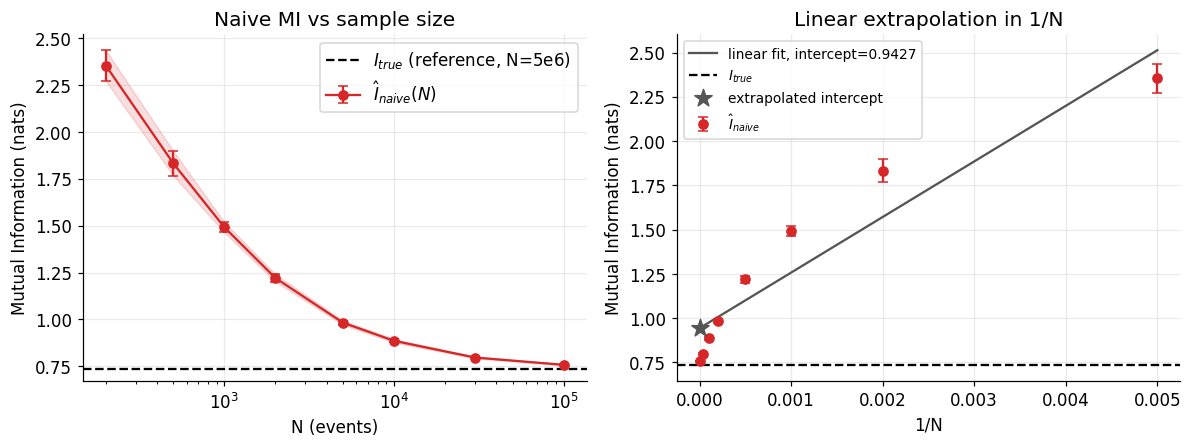
\includegraphics[width=\textwidth]{figs/fig02_bias_vs_N.png}
\caption{Left: naive $\hat I$ vs.\ sample size $N$, converging to the
reference value. Right: the same data plotted against $1/N$, with a linear
extrapolation to $1/N\to0$.}
\label{fig:bias-vs-N}
\end{figure}

% =============================================================================
\section{Corrections: Miller--Madow and shuffle-subtraction}
\label{sec:corrections}
% =============================================================================

\subsection{Miller--Madow correction}

The exact leading-order Miller--Madow correction \cite{Miller1955}
applies the $-(K-1)/(2N)$ term to \emph{each} of $S_A,S_B,S_{AB}$
separately and combines them:
\begin{equation}
\hat I_{MM} = \hat I_{\rm naive} - \frac{(K_{AB}-1)-(K_A-1)-(K_B-1)}{2N}
= \hat I_{\rm naive} - \frac{K_{AB}-K_A-K_B+1}{2N}.
\end{equation}
Crucially, $K_{AB}$ here must be the \emph{actually observed} number of
occupied joint bins, not the product $K_AK_B$: for correlated variables
(our case, by construction) the joint distribution concentrates on a
narrow ridge and $K_{AB}\ll K_AK_B$, so using the product in place of the
observed value wildly overcorrects and can drive $\hat I_{MM}$ negative.

\subsection{Shuffle-subtraction (label-permutation null)}

Randomly permuting the $B$-jet labels relative to the $A$-jet labels
\emph{within the same sample} destroys any true correlation
($I_{\rm true,shuffled}=0$ by construction) while reproducing the same
finite-sample bias. Averaging over many shuffles gives a direct empirical
estimate of the bias to subtract:
\begin{equation}
\hat I_{\rm corrected} = \hat I_{\rm naive} -
\big\langle \hat I_{\rm shuffled}\big\rangle .
\end{equation}
This makes no asymptotic assumption and remains reliable even when
$N\lesssim K_AK_B$, where Miller--Madow starts to break down. It has its
own bias, however: shuffling spreads the joint distribution over
\emph{more} bins than the true correlated data occupies, so the shuffled
surrogate is \emph{more} undersampled than the real data at the same $N$.
Shuffle-subtraction therefore tends to systematically
\textbf{overestimate} the bias and \textbf{overcorrect}, pulling
$\hat I_{\rm corrected}$ below $\Itrue$ when the true correlation is
strong.

\begin{table}[h]
\centering
\caption{Naive, Miller--Madow, and shuffle-corrected $\hat I$ vs.\ $N$.}
\label{tab:corrections}
\begin{tabular}{rrrrr}
\toprule
$N$ & $\hat I_{\rm naive}$ & $\hat I_{MM}$ & $\hat I_{\rm shuffle}$ & $\Itrue$ (ref.) \\
\midrule
200    & 2.2764 & 2.0889 & 0.0657 & 0.7329 \\
500    & 1.8694 & 1.6014 & 0.1436 & 0.7329 \\
1000   & 1.4271 & 1.1756 & 0.2422 & 0.7329 \\
2000   & 1.1873 & 0.9866 & 0.3809 & 0.7329 \\
5000   & 0.9766 & 0.8539 & 0.5592 & 0.7329 \\
20000  & 0.8259 & 0.7750 & 0.6792 & 0.7329 \\
\bottomrule
\end{tabular}
\end{table}

With the correct Miller--Madow formula (using the observed $K_{AB}$), both
corrections pull the small-$N$ estimates much closer to $\Itrue$ than the
naive value and stay well-behaved (no more diving negative). Neither lands
exactly on $\Itrue$ at very small $N$: Miller--Madow is only a
first-order truncation of the true bias expansion, and shuffle-subtraction
overcorrects when the true correlation is strong, as explained above. Both
effects shrink as $N$ grows.

The shuffle procedure gives more than a bias correction -- the spread of
$\hat I_{\rm shuffled}$ over many permutations \emph{is} the null
distribution for ``$\Itrue=0$'' at that $N$ and binning
(Fig.~\ref{fig:shuffle-null}). Plotting $\hat I_{\rm naive}$ against that
null distribution is a direct visual significance check: at $N=500$ the
null distribution itself is already centered well above zero (pure bias)
and the naive value sits close to or inside this null cloud, so on its own
it would not be significant evidence of correlation, even though the jets
are truly correlated by construction. By $N=20{,}000$ the null has
collapsed toward zero and the naive value clearly separates from it.

\begin{figure}[htb]
\centering
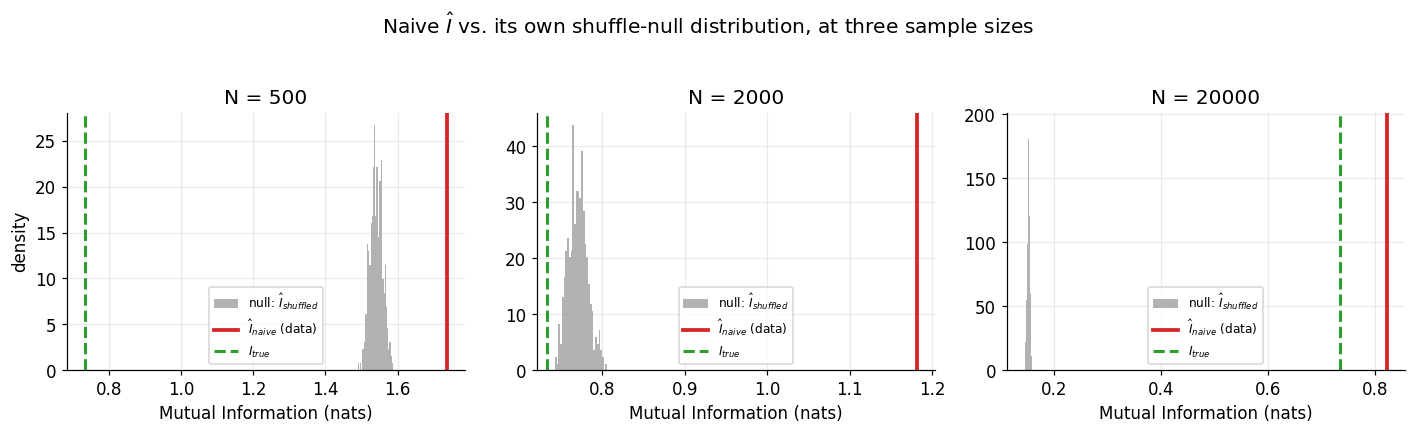
\includegraphics[width=\textwidth]{figs/fig03_shuffle_null.png}
\caption{Naive $\hat I$ (vertical line) against its own shuffle-null
distribution (histogram), at three sample sizes. Dashed line: true value.}
\label{fig:shuffle-null}
\end{figure}

Figure~\ref{fig:naive-vs-corrected} summarizes naive vs.\ corrected MI
across sample sizes, and Fig.~\ref{fig:residuals} plots
$|\hat I - \Itrue|$ on a log-log scale, which is the honest way to compare
convergence rates. Both corrections sit visibly below the naive curve at
fixed $N$; where the corrected residual curves run roughly parallel to the
naive curve rather than dropping faster, that indicates the residual error
is increasingly dominated by sub-leading bias terms that neither method
captures (Miller--Madow: higher-order $1/N^2,\ldots$ terms; shuffle: the
systematic overcorrection discussed above) -- exactly the gap the more
rigorous fix in Sec.~\ref{sec:nsb} is designed to close.

\begin{figure}[htb]
\centering
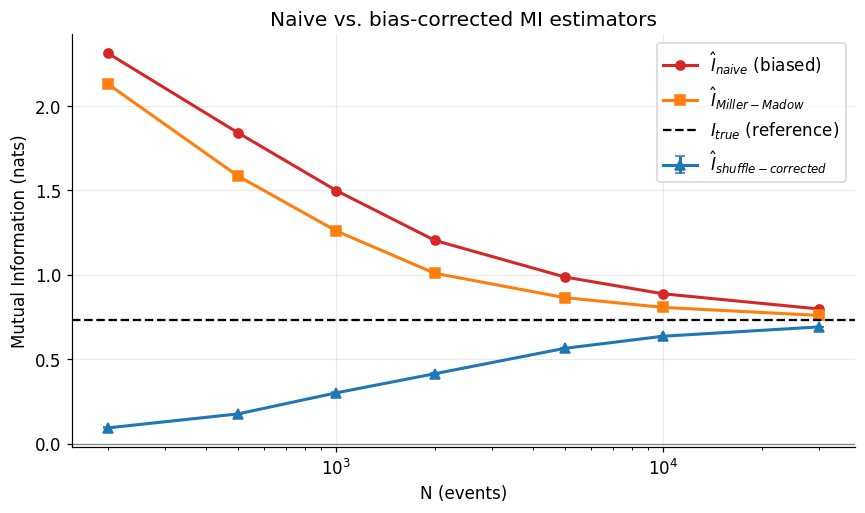
\includegraphics[width=0.75\textwidth]{figs/fig04_naive_vs_corrected.png}
\caption{Naive vs.\ bias-corrected MI estimators across sample sizes.}
\label{fig:naive-vs-corrected}
\end{figure}

\begin{figure}[htb]
\centering
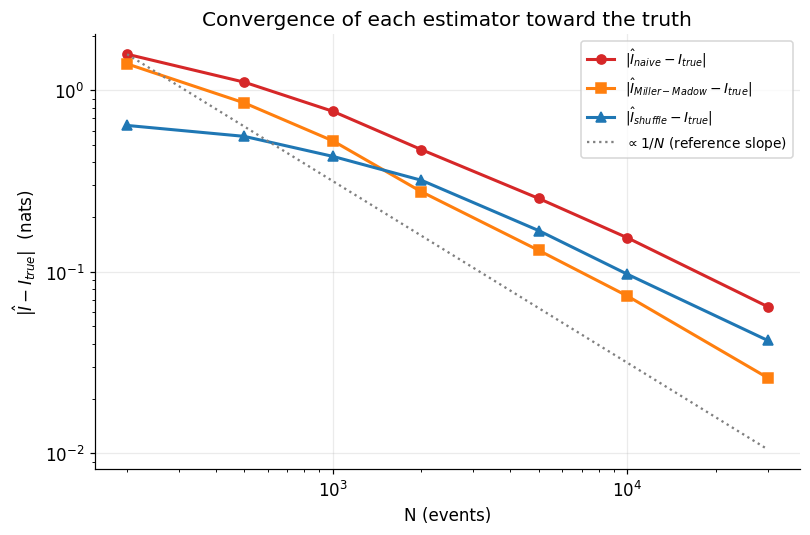
\includegraphics[width=0.75\textwidth]{figs/fig05_residual_convergence.png}
\caption{Convergence of each estimator toward the true value, on a log-log
scale, with a $1/N$ reference slope.}
\label{fig:residuals}
\end{figure}

% =============================================================================
\section{The rigorous fix: NSB Bayesian entropy estimator}
\label{sec:nsb}
% =============================================================================

Both corrections above are still, fundamentally, \textbf{point corrections
derived under a large-$N$ assumption} -- they estimate one number (the
bias) and subtract it. The \textbf{Nemenman--Shafee--Bialek (NSB)}
estimator \cite{NSB2002} takes a genuinely different approach: instead of
correcting a biased point estimate, it computes the \textbf{Bayesian
posterior mean entropy} directly, using a prior specifically constructed
to avoid smuggling in any implicit assumption about how spread-out the
distribution is. This is the standard tool for the severely-undersampled
regime ($N\lesssim K$) in the neuroscience spike-train MI literature --
precisely our regime once hadron multiplicities are binned in 2D.

The construction, in four steps:

\begin{enumerate}
\item Put a symmetric Dirichlet prior $P(p\,|\,\beta)\propto\prod_i
p_i^{\beta-1}$ over the $K$ possible bin probabilities. For any fixed
$\beta$, the posterior mean entropy given counts $\{n_i\}$ has a closed
form,
\begin{equation}
\langle S\rangle_{\beta,n} = \psi_0(N+K\beta+1) -
\sum_i \frac{n_i+\beta}{N+K\beta}\,\psi_0(n_i+\beta+1).
\end{equation}

\item \textbf{The catch:} a flat prior on $\beta$ does \emph{not} give a
flat prior on entropy -- for large $K$, $P(S\,|\,\beta)$ is sharply peaked
as a function of $\beta$. Fixing any single $\beta$ (as ordinary
add-one/Laplace/Jeffreys smoothing does) silently assumes an entropy value
before looking at the data.

\item NSB's fix: reweight $\beta$ by the hyperprior that makes the
\emph{induced} prior on $S$ flat -- literally the rate of change of the
prior mean entropy with $\beta$,
\begin{equation}
\rho(\beta) = K\,\psi_1(K\beta+1) - \psi_1(\beta+1).
\end{equation}

\item Average over $\beta$, weighted by both this hyperprior and the
Dirichlet--multinomial evidence $P(n\,|\,\beta)$,
\begin{equation}
\hat S_{\rm NSB} =
\frac{\int_0^\infty d\beta\;\rho(\beta)\,P(n\,|\,\beta)\,\langle
S\rangle_{\beta,n}}
{\int_0^\infty d\beta\;\rho(\beta)\,P(n\,|\,\beta)}.
\end{equation}
\end{enumerate}

This reduces to a tractable 1D numerical integral. We apply it separately
to $S_A,S_B,S_{AB}$ (each needs its own alphabet size $K$: for the joint
distribution, $K_{AB}^{\rm alphabet}=K_A^{\rm alphabet}\times K_B^{\rm
alphabet}$, the full product space of possible outcomes -- not the
observed $K_{AB}$ count from before, since NSB needs to know the size of
the space being integrated over, not how much of it happened to be hit),
then combine: $\hat I_{\rm NSB} = \hat S_A^{\rm NSB}+\hat S_B^{\rm
NSB}-\hat S_{AB}^{\rm NSB}$.

\begin{table}[h]
\centering
\caption{All four MI estimators, head to head.}
\label{tab:all-estimators}
\begin{tabular}{rrrrrr}
\toprule
$N$ & $\hat I_{\rm naive}$ & $\hat I_{MM}$ & $\hat I_{\rm shuffle}$ &
$\hat I_{\rm NSB}$ & $\Itrue$ (ref.) \\
\midrule
200   & 2.3511 & 2.1711 & 0.0578 & 0.5098 & 0.7329 \\
500   & 1.7525 & 1.5035 & 0.2137 & 0.6833 & 0.7329 \\
1000  & 1.5071 & 1.2711 & 0.3062 & 0.7369 & 0.7329 \\
2000  & 1.2299 & 1.0367 & 0.4340 & 0.7416 & 0.7329 \\
5000  & 1.0030 & 0.8842 & 0.5807 & 0.7678 & 0.7329 \\
20000 & 0.8222 & 0.7716 & 0.6752 & 0.7411 & 0.7329 \\
\bottomrule
\end{tabular}
\end{table}

NSB tracks $\Itrue$ closely across the entire range, including at
$N=200$ where the naive estimator is off by roughly a factor of three and
Miller--Madow has barely moved. This is the payoff of treating the whole
problem as Bayesian inference over entropy rather than patching a biased
point estimate after the fact. Figure~\ref{fig:nsb-comparison} adds NSB to
the convergence comparison: its residual curve sits visibly below the
other three methods across most of the range, and in particular stays far
more stable at small $N$ -- it doesn't need $N\gg K$ to behave sensibly.

\begin{figure}[htb]
\centering
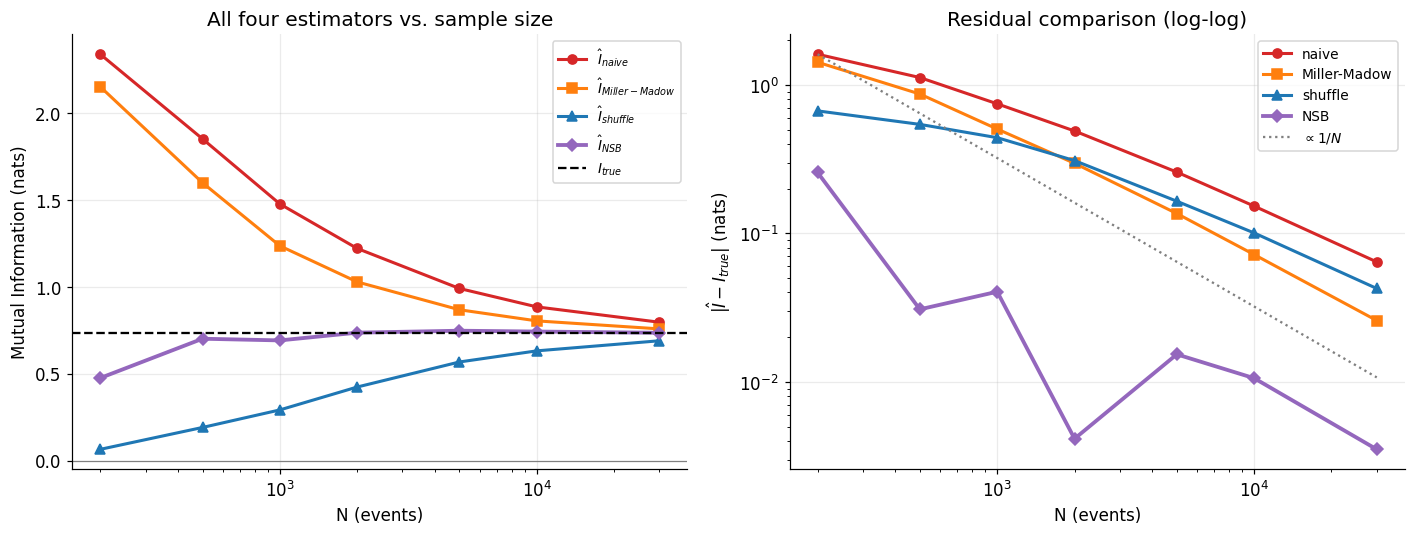
\includegraphics[width=\textwidth]{figs/fig06_nsb_comparison.png}
\caption{Left: all four estimators vs.\ sample size. Right: residual
comparison on a log-log scale, with a $1/N$ reference slope.}
\label{fig:nsb-comparison}
\end{figure}

\paragraph{Practical notes for the real STAR dijet data.}
\begin{itemize}
\item The alphabet size $K$ (for each marginal, and $K_A\times K_B$ for
the joint) needs to be fixed \emph{before} looking at the data -- pick a
generous fixed upper bound on plausible hadron multiplicity per jet
(e.g.\ from detector acceptance / kinematic limits), not the observed
range, or a data-dependent bias is reintroduced through the back door.
\item NSB is somewhat more expensive per call than MM or
shuffle-subtraction (a 1D numerical integral instead of a closed-form
correction or a handful of permutations), but it remains a fraction of a
second per event sample -- entirely practical for a real analysis,
including a full jackknife or bootstrap for uncertainty quantification.
\item The same estimator applies directly to $\SBA=S_{AB}-S_A$ and to
$\NMI$ -- swap in the NSB entropies there instead of the
naive/MM/shuffle versions before quoting any central value of these
derived quantities.
\end{itemize}

% =============================================================================
\section{Summary and recommendations from the toy Monte Carlo study}
% =============================================================================

\begin{enumerate}

\item \textbf{The observables are classically bounded, and the bounds are
not testable physics.} $\SBA\geq0$ and $\NMI\leq1$ hold identically for
any measured multiplicity distribution (Sec.~\ref{sec:nogo}); they cannot
be used as quantum witnesses. The physically meaningful measurements are
the central values themselves -- $I(A{:}B)$, $\NMI$, $\SBA$ -- compared
across kinematics, against generator baselines, and against
entanglement-ansatz predictions (Sec.~\ref{sec:motivation}); proximity to
the perfect-correlation limit $\NMI\to1$ is the Schmidt-limit signature,
not a bound violation. Genuine quantum discord likewise cannot be
computed from hadron-count histograms -- any classical joint distribution
gives discord $\equiv0$ (Sec.~\ref{sec:observable}).

\item \textbf{The naive plug-in MI estimator is always biased upward},
with leading term $\approx(K_{AB}-K_A-K_B+1)/(2N)$. Finer binning or
fewer events both make it worse -- comparing different STAR running
periods, luminosities, or binning choices will report different central
MI values from what should be the same physics, purely from this effect.

\item \textbf{Miller--Madow} (done correctly, using the observed
$K_{AB}$, not the product $K_AK_B$) and \textbf{shuffle-subtraction} both
substantially reduce this bias and stay well-behaved, but neither is exact
at small $N$: Miller--Madow is a first-order truncation;
shuffle-subtraction tends to systematically overcorrect when the true
correlation is strong.

\item \textbf{NSB} is the recommended estimator for the real analysis: a
Bayesian posterior-mean entropy built on a prior specifically constructed
to be uninformative about entropy itself. It tracks the truth closely
across the entire tested $N$ range, including deep in the
severely-undersampled regime where the other methods struggle, at a
modest computational cost.

\item \textbf{Before quoting any measured correlation} -- especially one
to be compared across datasets or against model predictions --
bias-correct with NSB and validate the quoted uncertainty against the
estimator's own sampling noise floor at that $N$, obtained by
bootstrap/jackknife on the dataset itself and calibrated by a closure
test at the analysis's actual statistics (Sec.~\ref{sec:closure}).

\item \textbf{Any estimated $\widehat{\SBA}<0$ or $\widehat{\NMI}>1$, at
any apparent significance, is a finite-sample artifact by theorem}
(Sec.~\ref{sec:nogo}). Its appearance is a diagnostic of residual
estimator bias or underestimated uncertainty, not of physics; the correct
response is more statistics or better correction, not interpretation.

\end{enumerate}

% =============================================================================
\section{Validation on PYTHIA~8 Monte Carlo simulation}
\label{sec:pythia}
% =============================================================================

The toy model of Secs.~\ref{sec:toymc}--\ref{sec:nsb} demonstrates that the
estimator pipeline behaves correctly on data with a known, simple
generative structure. The natural next step is to check the same pipeline
on a full QCD event generator, where hadron multiplicities arise from
parton showering, hadronization, and (optionally) the underlying event --
none of which was built into the toy model by hand. We generated
back-to-back charged-jet dijets with PYTHIA~8 (Monash 2013 tune,
anti-$k_T$ jets, $R=0.4$, charged final-state particles only, matching a
STAR-TPC-like charged-jet definition) and applied the identical naive/
Miller--Madow/shuffle/NSB pipeline, unmodified, to the generator output.
% TODO (reproducibility): document here the PYTHIA version number, the
% hard-process selection and pT-hat range, the jet pT thresholds and
% |eta| acceptance, the back-to-back Delta-phi selection, and the
% multiplicity binning / alphabet bounds used for NSB.

This particular validation run used LHC-like kinematics
($\sqrt{s}=14$~TeV rather than the $\sqrt{s}=200$~GeV RHIC energy that
motivates the eventual STAR measurement) specifically \emph{because} of
its much wider accessible jet-$p_T$ range: as discussed below
(Sec.~\ref{sec:pythia-ptdep}), the multiplicity-vs-$p_T$ correlation
predicted by QCD is intrinsically a slow, logarithmic effect, and a wide
dynamic range makes it far easier to confirm the pipeline is tracking real
physics rather than an artifact of a narrow kinematic window. The $200$~GeV
run for the actual STAR measurement is a separate, ongoing exercise (see
Sec.~\ref{sec:conclusions}); everything in this section is a
\emph{methods validation}, not a physics result.

\subsection{Multiplicity and $p_T$ distributions}

Figure~\ref{fig:py-mult-dist} shows the charged-multiplicity distributions
for the leading and subleading jets, overlaid with a method-of-moments
Negative-Binomial fit (as in Sec.~\ref{sec:toymc}). Both jets show genuine
overdispersion relative to Poisson (var/mean $=1.55$ for the leading jet,
$1.29$ for the subleading jet), qualitatively consistent with -- though
not identical in shape to -- the NBD-like multiplicity distributions
assumed in the toy model. This is a useful cross-check in its own right:
the toy model's central structural assumption (NBD-shaped marginals) is
not merely a convenient fiction, but a reasonable approximation to what a
full QCD generator actually produces.

\begin{figure}[htb]
\centering
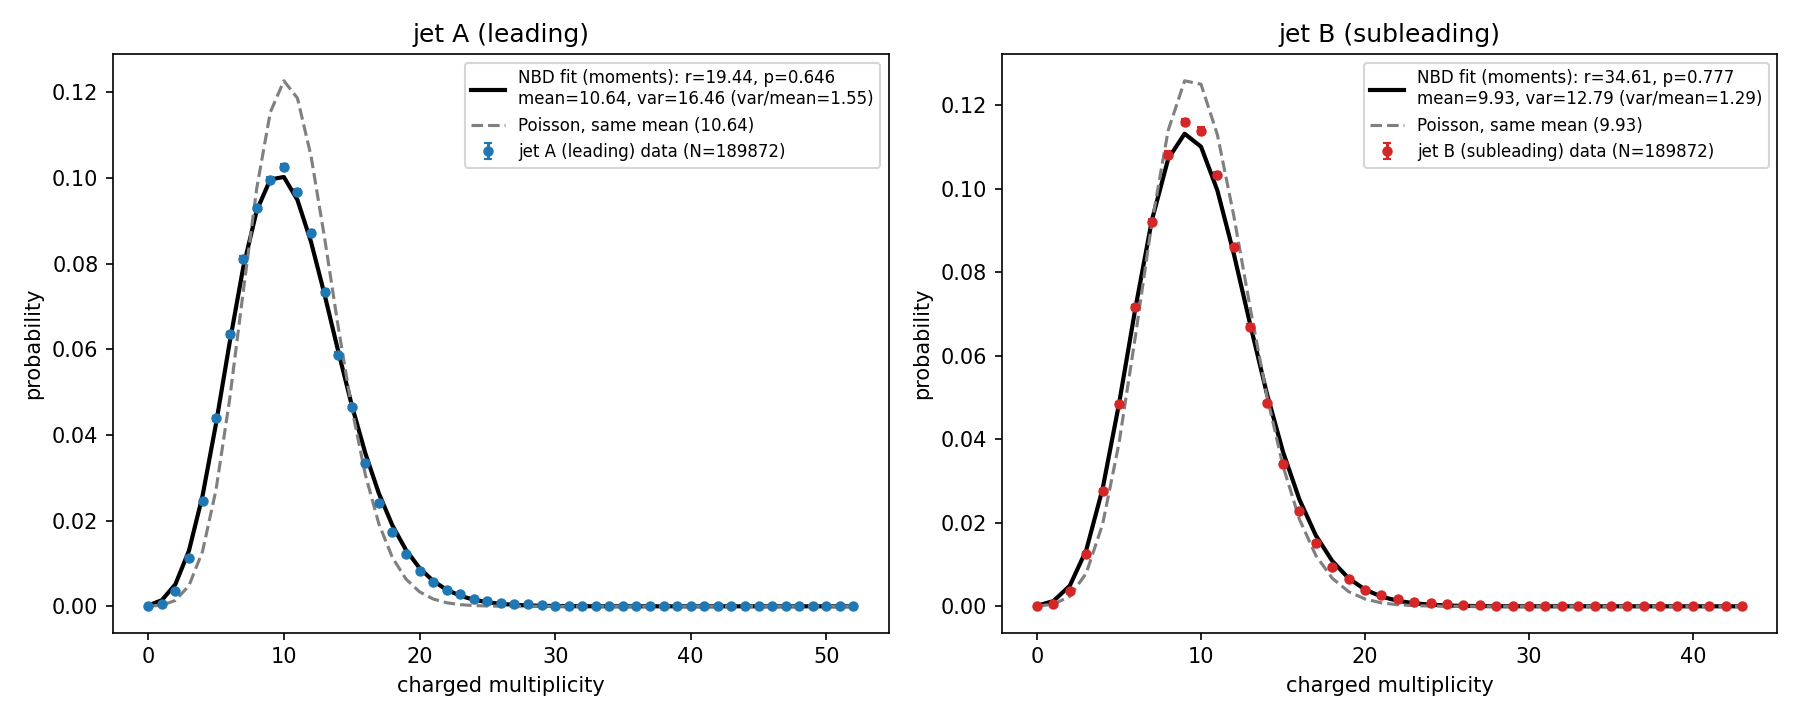
\includegraphics[width=\textwidth]{figs/dijet_entropy_result_truth_multiplicity_dists.png}
\caption{PYTHIA~8: charged-multiplicity distributions for the leading
(left) and subleading (right) jet, with NBD and same-mean Poisson overlay
(cf.\ the toy-model version, Sec.~\ref{sec:toymc}).}
\label{fig:py-mult-dist}
\end{figure}

Figure~\ref{fig:py-joint-mult} shows the corresponding joint distribution:
36.9\% of the $53\times44$ grid is occupied ($K_{AB}=861$) at
$N\approx1.9\times10^5$ events -- a moderately, not severely, undersampled
regime, comparable to the middle of the range explored in the toy study.
Figure~\ref{fig:py-pt-dist} shows the (steeply falling, as expected for a
QCD jet spectrum) leading- and subleading-jet $p_T$ distributions, and
Fig.~\ref{fig:py-joint-pt} their joint distribution -- the latter makes
visually clear why quantile (rather than fixed-width) $p_T$ binning is
necessary for the differential measurements below: the bulk of events sit
in a narrow low-$p_T$ band, with a long, sparse tail.

\begin{figure}[htb]
\centering
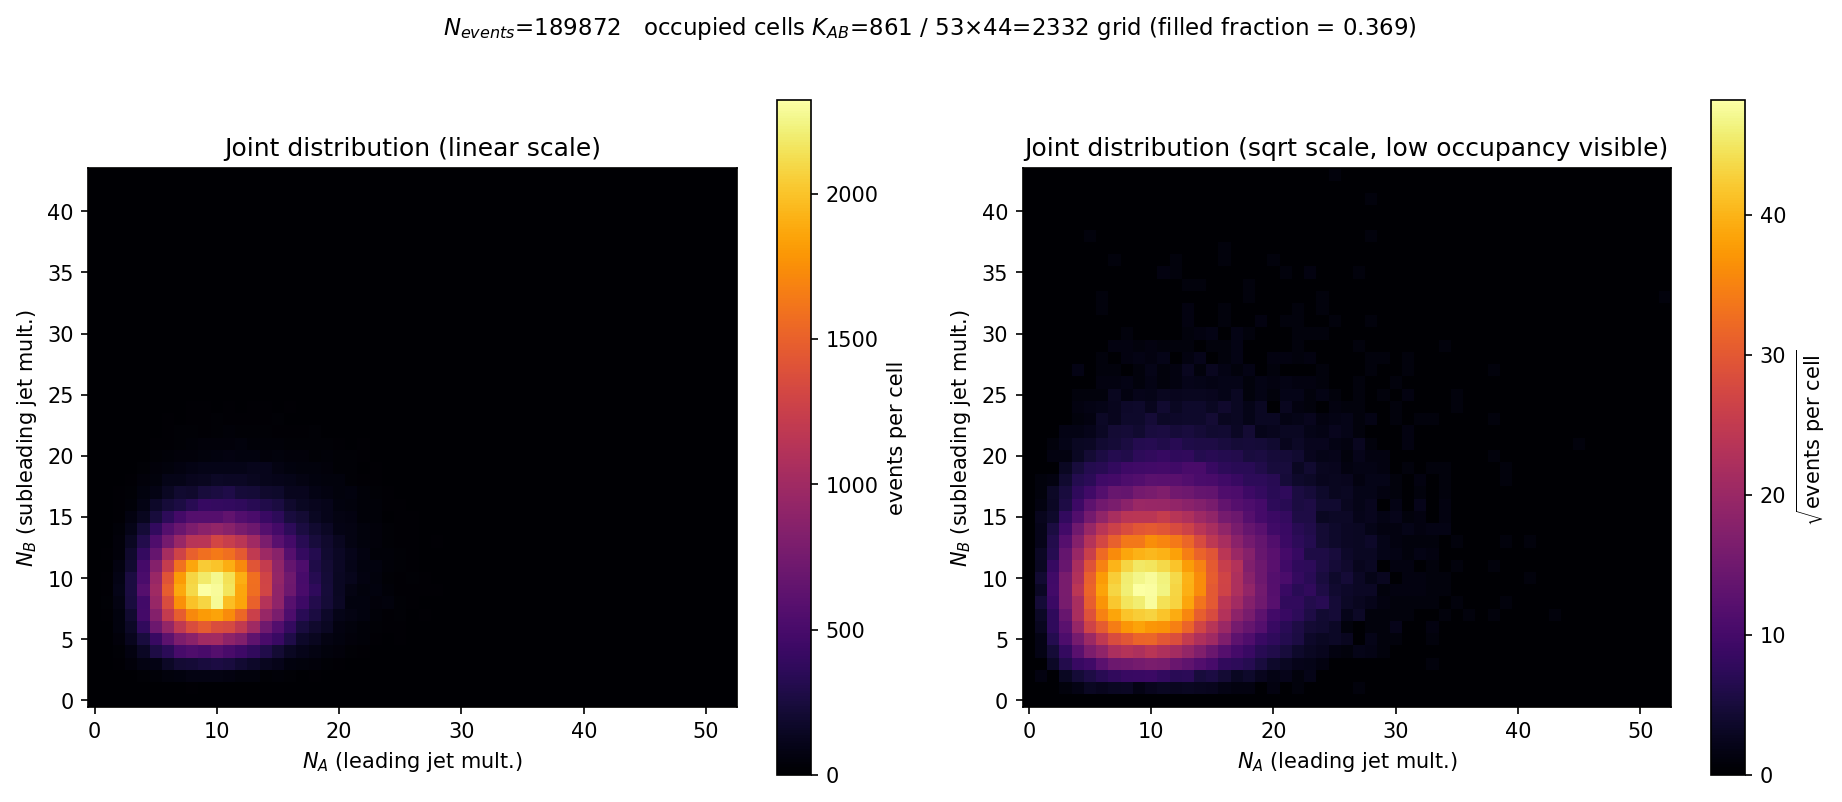
\includegraphics[width=0.85\textwidth]{figs/dijet_entropy_result_truth_joint_multiplicity_dist.png}
\caption{PYTHIA~8: joint charged-multiplicity distribution, linear and
sqrt color scale (cf.\ Fig.~\ref{fig:marginals-joint}).}
\label{fig:py-joint-mult}
\end{figure}

\begin{figure}[htb]
\centering
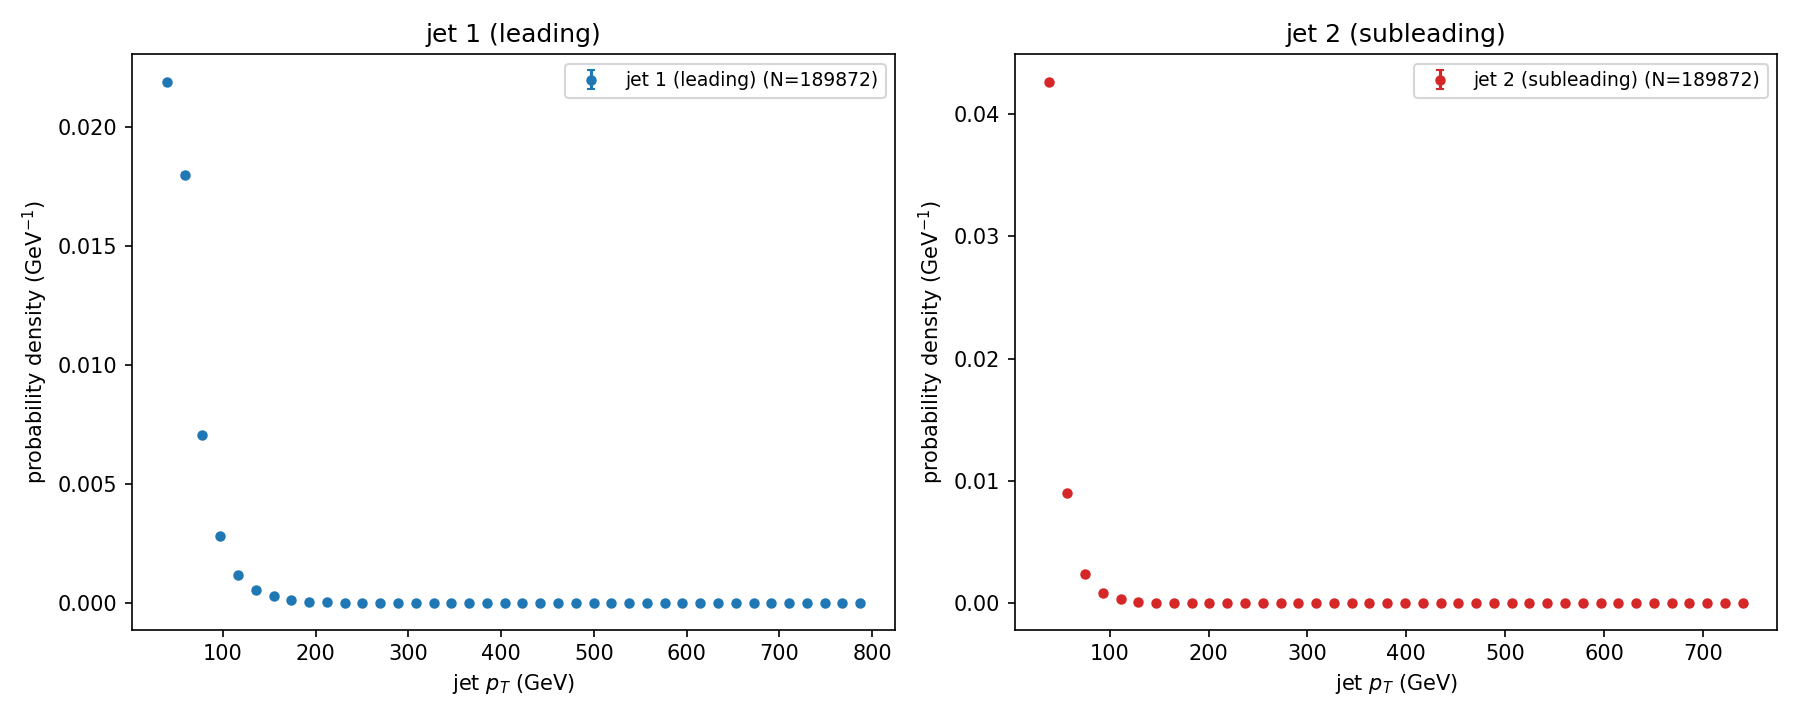
\includegraphics[width=\textwidth]{figs/dijet_entropy_result_truth_pt_dists.png}
\caption{PYTHIA~8: leading- and subleading-jet $p_T$ distributions.}
\label{fig:py-pt-dist}
\end{figure}

\begin{figure}[htb]
\centering
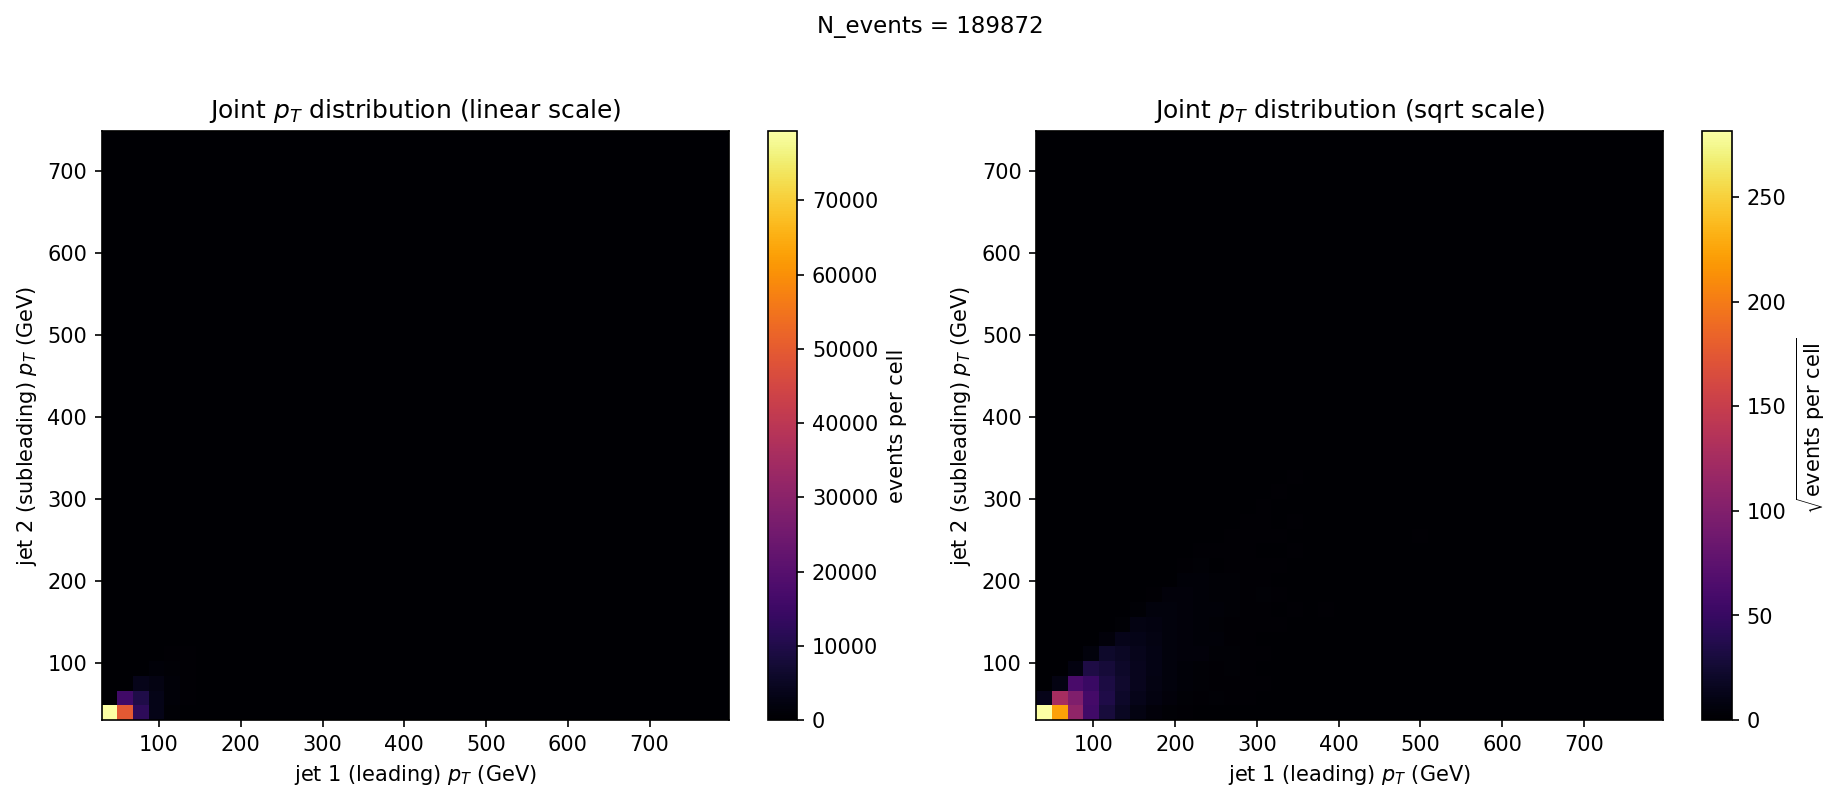
\includegraphics[width=0.85\textwidth]{figs/dijet_entropy_result_truth_joint_pt_dist.png}
\caption{PYTHIA~8: joint leading/subleading jet $p_T$ distribution,
linear and sqrt color scale.}
\label{fig:py-joint-pt}
\end{figure}

\subsection{The multiplicity--$p_T$ correlation}
\label{sec:pythia-ptdep}

A basic physical expectation -- confirmed experimentally (e.g.\ ALICE
\cite{ALICE2024jets}: ``the mean charged-particle multiplicity inside the
leading jet cone rises monotonically with increasing jet $p_T$'') -- is
that higher-$p_T$ jets should carry higher charged multiplicity, via
additional phase space for parton radiation before hadronization. This
growth is predicted by QCD coherent-branching (MLLA) arguments
\cite{DKMT1991} to be slow and roughly \emph{logarithmic} in $p_T$, not
linear, which matters directly for how easy the effect is to see over a
limited kinematic range (as it was, initially, in an earlier $200$~GeV
validation attempt with a narrower accessible $p_T$ window).

Figure~\ref{fig:py-mult-vs-pt} shows the raw, unbinned-by-any-entropy-
machinery profile of mean charged multiplicity vs.\ jet $p_T$, together
with a weighted fit of the MLLA-motivated form $\langle N\rangle = a +
b\ln p_T$. The fitted slope is highly significant for both jets ($b =
3.77\pm0.05$, $83\sigma$, leading jet; $b=4.71\pm0.07$, $66\sigma$,
subleading jet) -- direct, quantitative confirmation that PYTHIA~8
reproduces the expected QCD multiplicity-growth pattern, and that the
analysis pipeline correctly recovers it from generator output with no
prior assumption beyond bin means and standard errors.

\begin{figure}[htb]
\centering
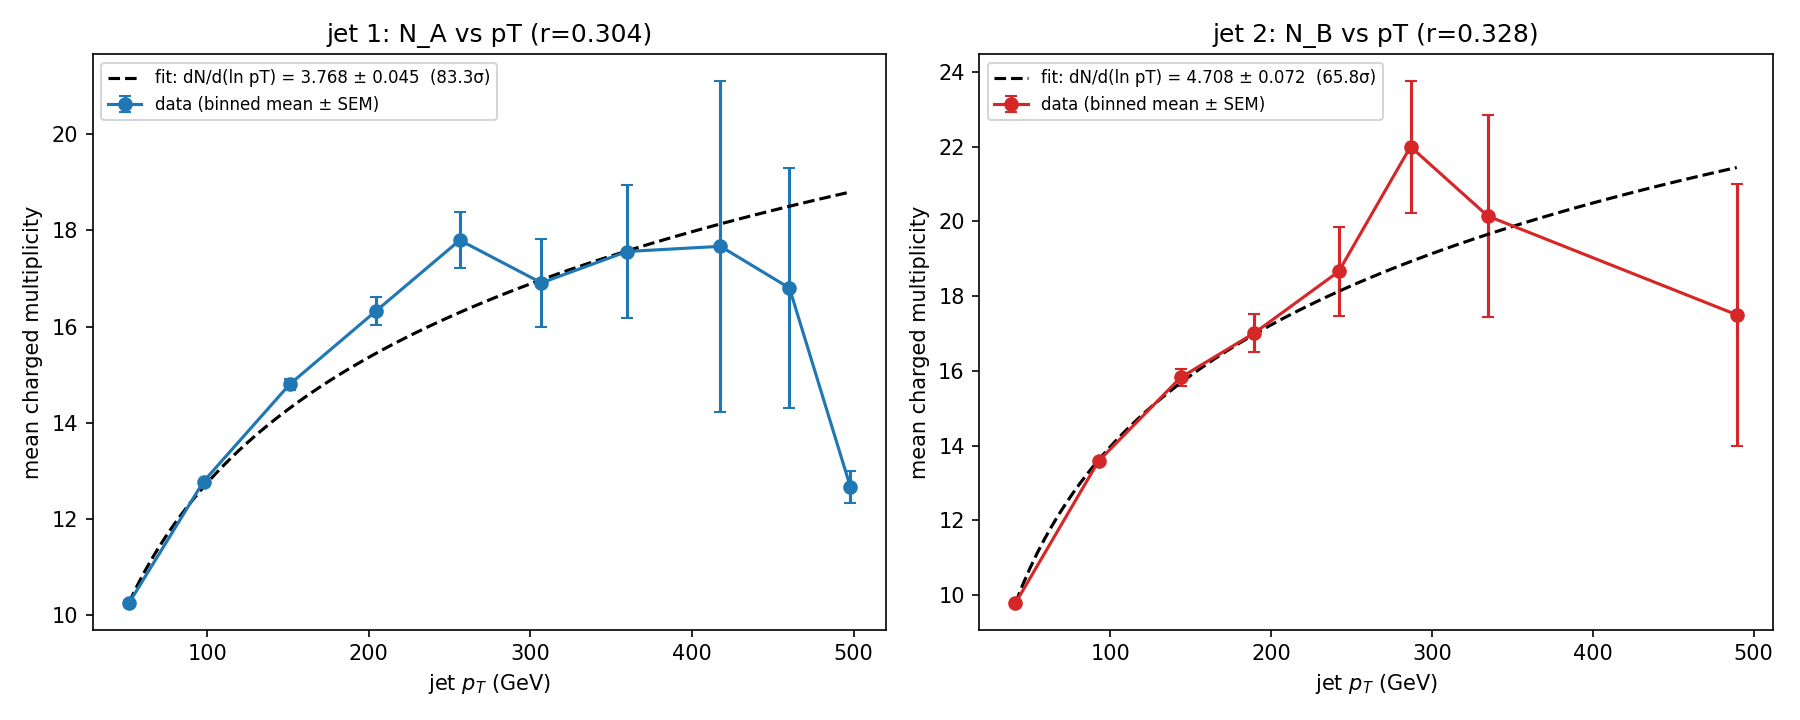
\includegraphics[width=\textwidth]{figs/dijet_entropy_result_truth_mult_vs_pt_profile.png}
\caption{PYTHIA~8: raw mean charged multiplicity vs.\ jet $p_T$ (binned
mean $\pm$ SEM), with a weighted fit to $\langle N\rangle=a+b\ln p_T$.
Both slopes are significant at $>60\sigma$.}
\label{fig:py-mult-vs-pt}
\end{figure}

\subsection{Finite-sample bias, reproduced on generator output}

Figure~\ref{fig:py-bias-scan} repeats the toy study's core diagnostic
(Sec.~\ref{sec:toymc}) directly on subsamples of the real PYTHIA~8 output:
the naive $\hat I$ falls from $\approx0.66$~nats at $N=200$ down toward
the full-sample NSB value ($\approx0.009$~nats) as $N$ grows to
$\approx1.9\times10^5$ -- the same qualitative bias curve seen throughout
Sec.~\ref{sec:toymc}, now confirmed on a dataset the toy model was never
built to resemble. This is a meaningful cross-check: the bias mechanism
identified analytically (Sec.~\ref{sec:bias}) and demonstrated on a
synthetic Gamma-Poisson model is not an artifact of that specific
generative structure -- it appears with the same shape on genuine QCD
Monte Carlo output.

\begin{figure}[htb]
\centering

\includegraphics[width=0.8\textwidth]{figs/dijet_entropy_result_truth_bias_scan.png}
\caption{PYTHIA~8: naive $\hat I$ vs.\ subsample size $N$, real generator
output (cf.\ the toy-model version, Fig.~\ref{fig:bias-vs-N}).}
\label{fig:py-bias-scan}
\end{figure}

\subsection{Point estimates on the full sample}

Figure~\ref{fig:py-summary} shows all four estimators on the full sample
($N\approx1.9\times10^5$): naive ($0.0112\pm0.0004$), Miller--Madow
($0.0092\pm0.0004$), shuffle-corrected ($0.0084\pm0.0003$), and NSB
($0.0085\pm0.0004$~nats) -- naive sits visibly above the other three, as
expected from the bias mechanism above, while Miller--Madow/shuffle/NSB
agree closely with each other, consistent with all three having converged
toward the true value at this statistics (matching the closure seen among
independently-biased estimators at large $N$ in the toy study,
Sec.~\ref{sec:toymc}). The conditional entropy $\SBA=2.65$~nats and
$\NMI\ll1$ sit far from the perfect-correlation (Schmidt-limit)
boundary: PYTHIA~8's cross-jet multiplicity correlation is weak on the
$\NMI$ scale. Since PYTHIA's hadronization contains no entanglement by
construction, these values constitute the classical QCD generator
baseline of Sec.~\ref{sec:motivation} against which the same measurement
on real data can eventually be compared. This measurement is a validation
of the estimator machinery, not a physics claim.

\begin{figure}[htb]
\centering
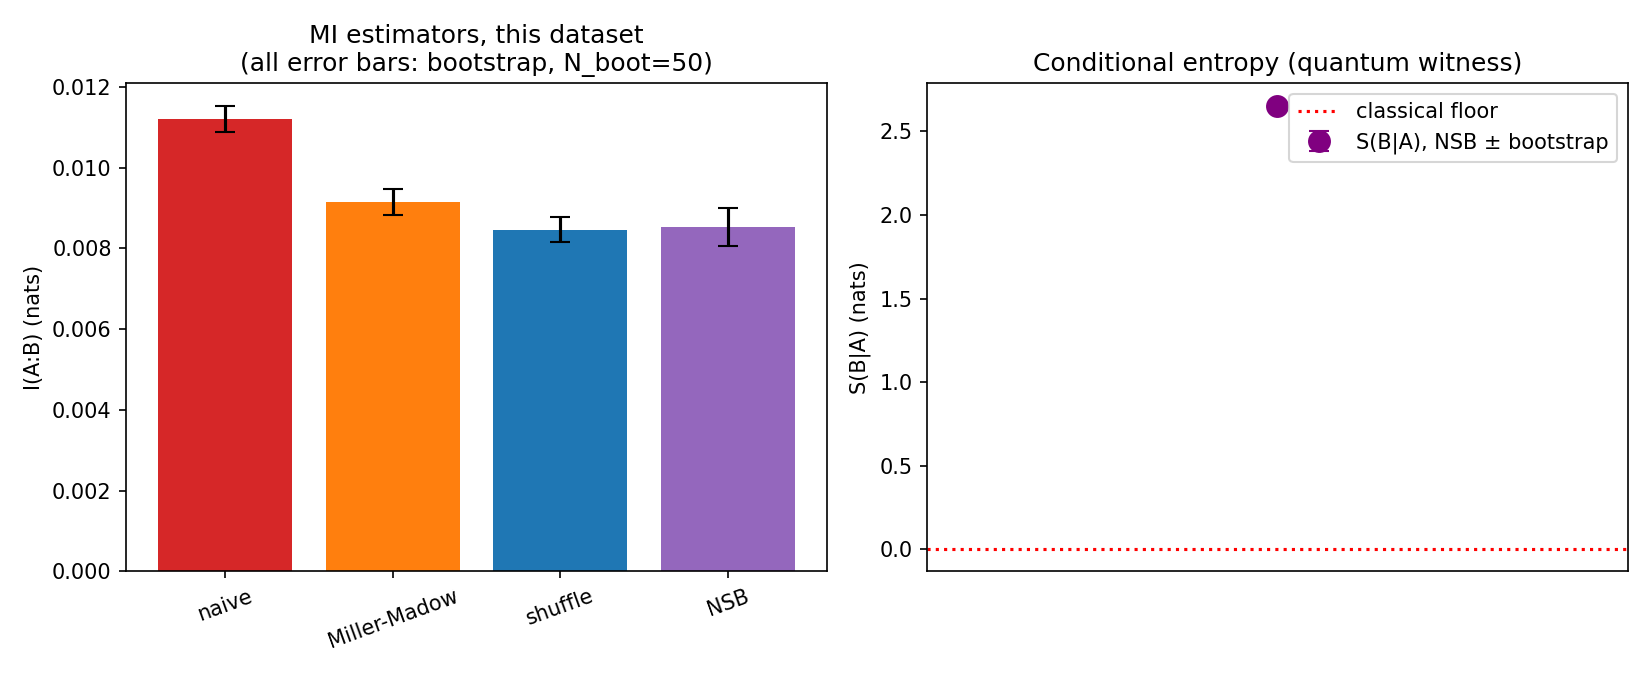
\includegraphics[width=\textwidth]{figs/dijet_entropy_result_truth_summary.png}
\caption{PYTHIA~8: all four MI estimators (left) and $\SBA$ (right) on
the full sample, bootstrap error bars.}
\label{fig:py-summary}
\end{figure}

\subsection{Differential measurement vs.\ jet $p_T$}

Figures~\ref{fig:py-entropy-pt}--\ref{fig:py-sba-pt} show $S_A,S_B,S_{AB}$,
$I(A{:}B)$, and $\SBA$ (NSB) in quantile bins of leading-jet $p_T$. All
three entropies rise smoothly with $p_T$ (Fig.~\ref{fig:py-entropy-pt}),
directly reflecting the multiplicity growth of Sec.~\ref{sec:pythia-ptdep}.
$I(A{:}B)$ (Fig.~\ref{fig:py-mi-pt}) also rises with $p_T$, modestly at
low-to-mid $p_T$ and more sharply in the highest (widest, most
statistics-limited) bin; $\SBA$ (Fig.~\ref{fig:py-sba-pt}) stays solidly
positive and rising throughout, i.e.\ the correlation stays far from the
perfect-correlation boundary at every $p_T$ probed.

\begin{figure}[htb]
\centering
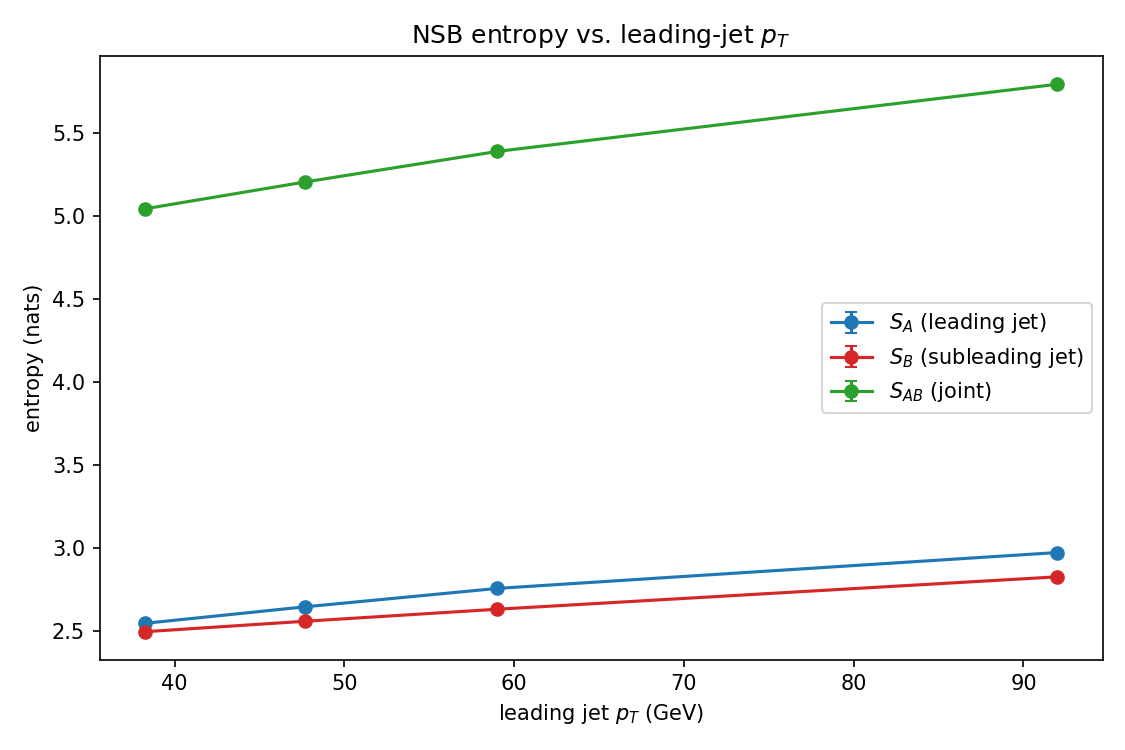
\includegraphics[width=\textwidth]{figs/dijet_entropy_result_truth_entropy_vs_pt.png}
\caption{PYTHIA~8: $S_A,S_B,S_{AB}$ (NSB) vs.\ leading-jet $p_T$.}
\label{fig:py-entropy-pt}
\end{figure}

\begin{figure}[htb]
\centering
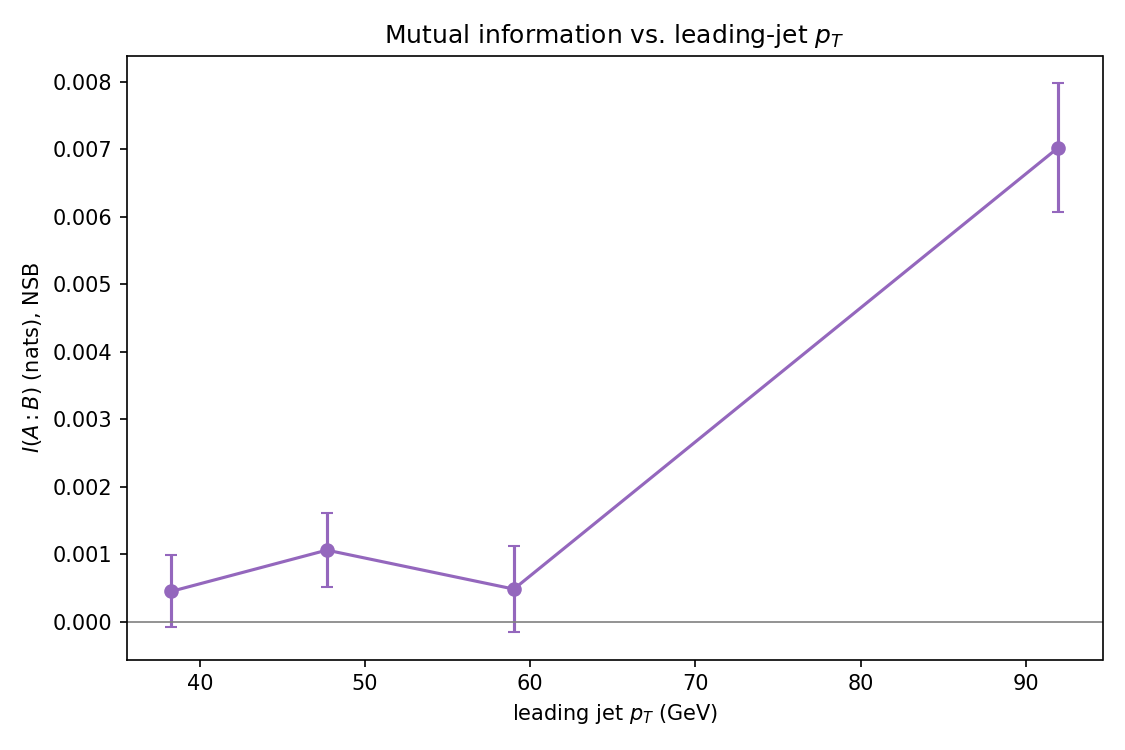
\includegraphics[width=0.8\textwidth]{figs/dijet_entropy_result_truth_MI_vs_pt.png}
\caption{PYTHIA~8: $I(A{:}B)$ (NSB) vs.\ leading-jet $p_T$.}
\label{fig:py-mi-pt}
\end{figure}

\begin{figure}[htb]
\centering
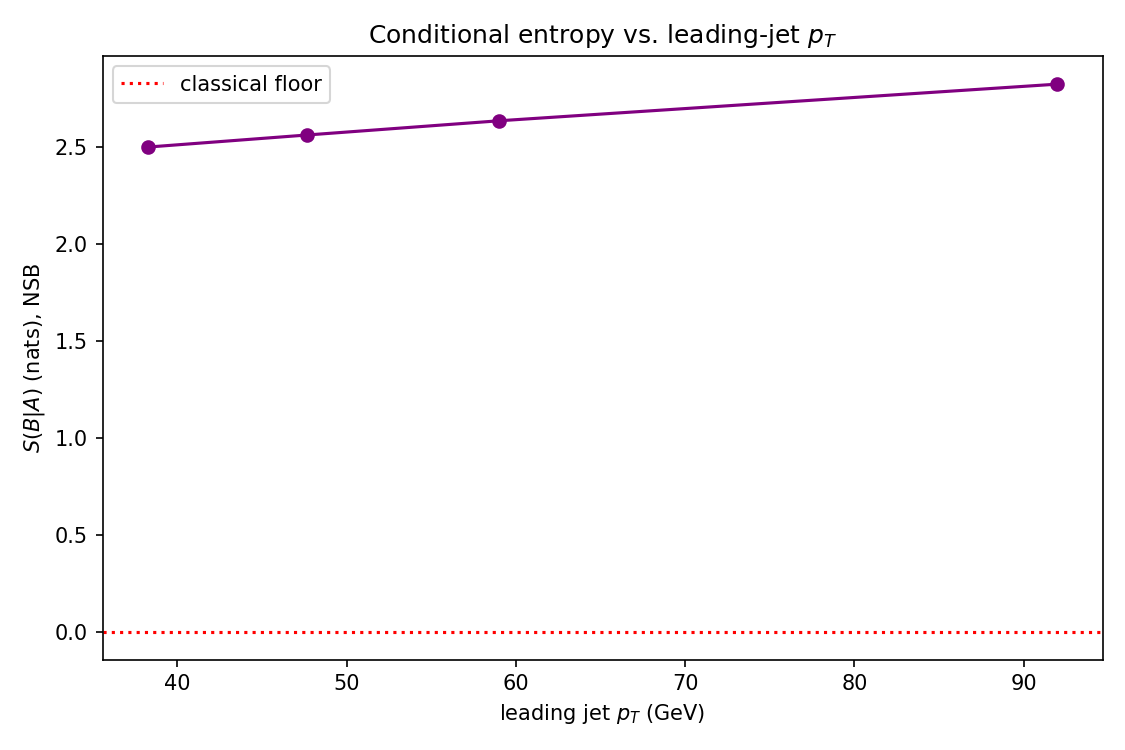
\includegraphics[width=0.8\textwidth]{figs/dijet_entropy_result_truth_SBA_vs_pt.png}
\caption{PYTHIA~8: $\SBA$ (NSB) vs.\ leading-jet $p_T$.}
\label{fig:py-sba-pt}
\end{figure}

\subsection{Multi-method comparison vs.\ $p_T$}

Figure~\ref{fig:py-method-comparison} overlays naive/Miller--Madow/
shuffle/NSB for $I(A{:}B)$, and naive/Miller--Madow/NSB for $\SBA$ (no
shuffle analogue, Sec.~\ref{sec:nsb}), each with bootstrap error bars
computed by the same unified procedure (Sec.~\ref{sec:pitfall}). The
bias hierarchy naive~$>$~Miller--Madow~$\gtrsim$~NSB~$\approx$~shuffle
seen on the full sample (Fig.~\ref{fig:py-summary}) persists across
$p_T$ bins, most visibly in the highest-$p_T$ (lowest-statistics) bin,
where naive's upward bias is largest -- exactly the pattern the toy study
predicts for a bin with fewer events and a wider effective alphabet.

\begin{figure}[htb]
\centering
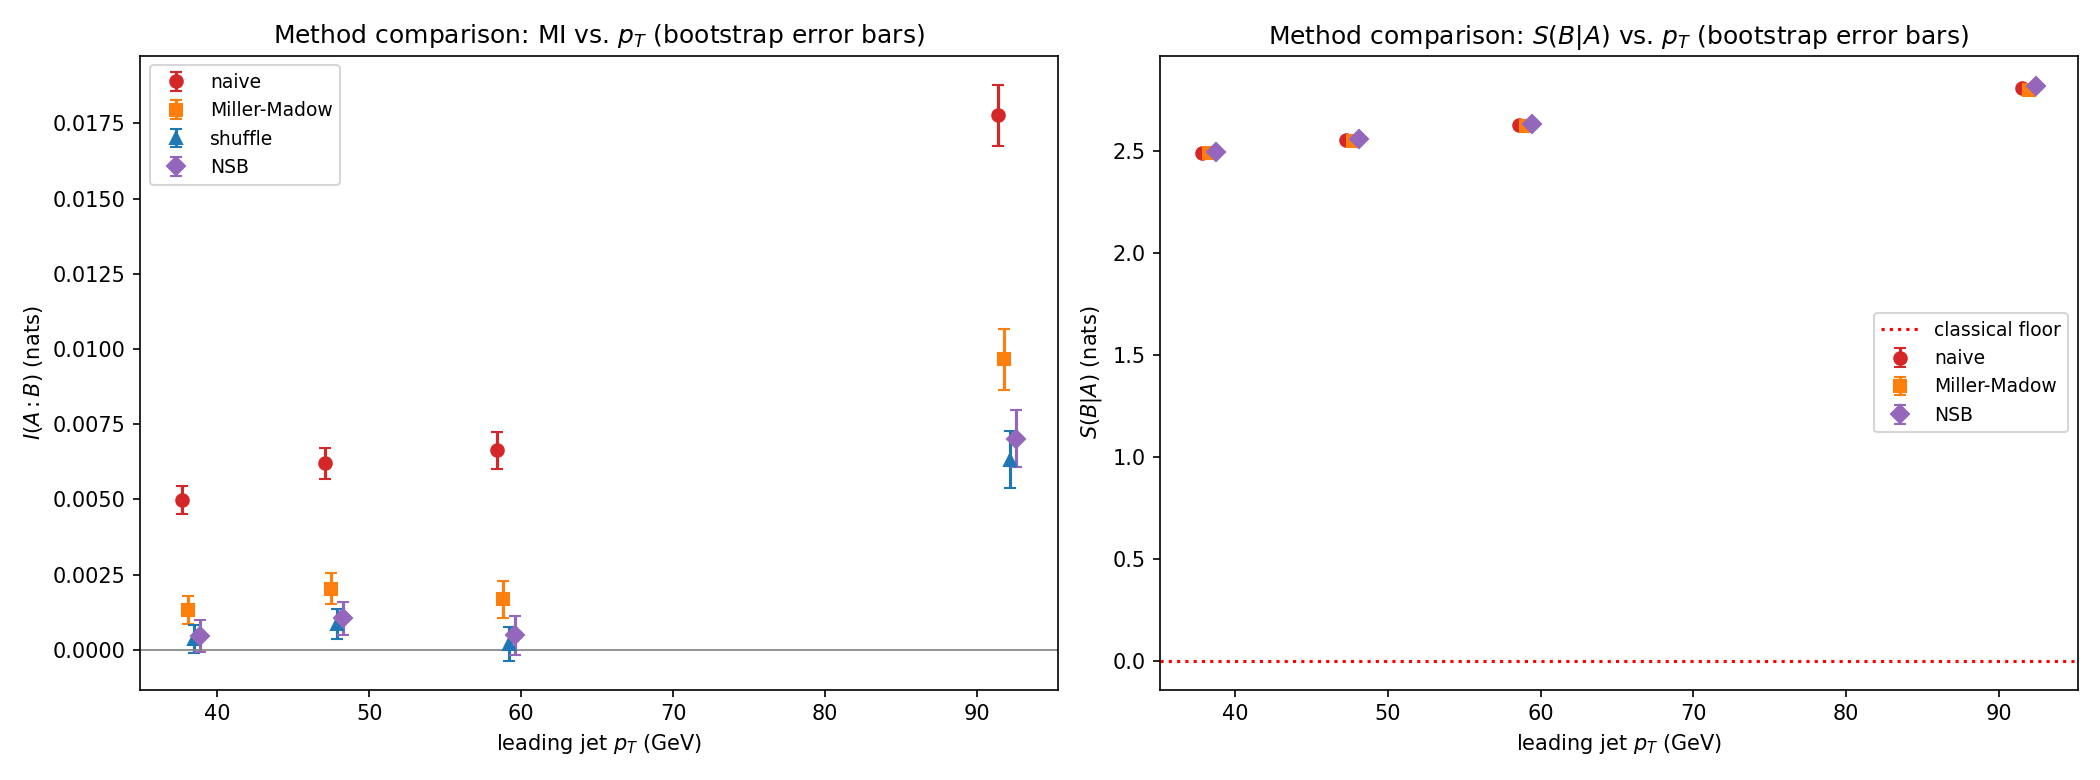
\includegraphics[width=\textwidth]{figs/dijet_entropy_result_truth_method_comparison_vs_pt.png}
\caption{PYTHIA~8: method comparison for $I(A{:}B)$ (left) and $\SBA$
(right) vs.\ leading-jet $p_T$, bootstrap error bars throughout.}
\label{fig:py-method-comparison}
\end{figure}

\subsection{Cross-validation with an independent implementation, and
normalized mutual information}
\label{sec:pythia-nmi}

The full pipeline was re-implemented independently in ROOT/C++ (with its
own validated digamma/trigamma special functions, NSB posterior
computation, and bootstrap machinery) as a cross-check against the
Python implementation above, applied to the \emph{same} generated event
sample ($N\approx1.9\times10^5$, identical to
Secs.~\ref{sec:pythia}--\ref{sec:pythia-ptdep}). This section reports the
ROOT pipeline's results for $\NMI$ (Sec.~\ref{sec:observable}), which
were not part of the original Python-only analysis above.

Figure~\ref{fig:py-nmi-pt} shows $\NMI$ (NSB) vs.\ leading-jet $p_T$: all
values sit at $\NMI\ll1$, far below the perfect-correlation bound,
consistent with the small $I(A{:}B)$ values already seen in absolute
terms (Fig.~\ref{fig:py-mi-pt}) and, as before, expected for a classical
event generator with weak cross-jet correlation. The value of $\NMI$ here
is methodological rather than a physics result on this dataset: it
demonstrates the normalized observable is measurable with the same NSB
machinery as $I$ and $\SBA$, and (Sec.~\ref{sec:pitfall} below) that
doing so correctly requires some care.

\begin{figure}[htb]
\centering
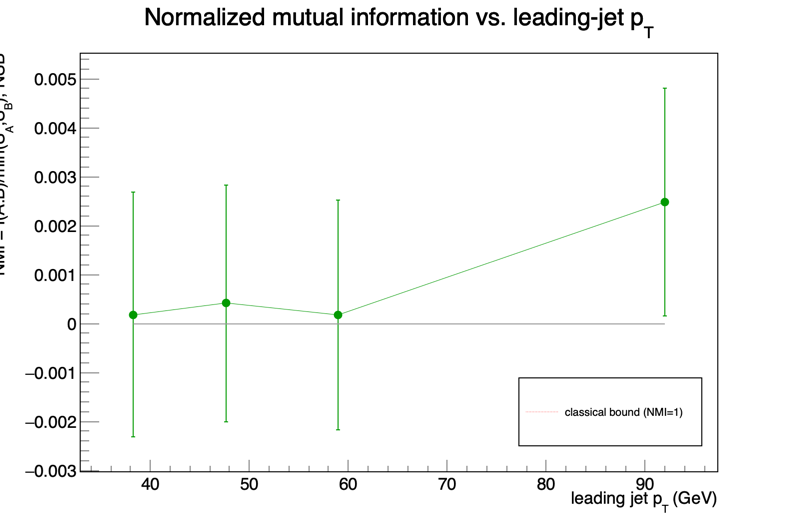
\includegraphics[width=0.8\textwidth]{figs/root_NMI_vs_pt.png}
\caption{PYTHIA~8 (ROOT implementation): $\NMI=I(A{:}B)/\min(S_A,S_B)$
(NSB) vs.\ leading-jet $p_T$. All values are far below the
perfect-correlation bound $\NMI=1$, as expected for a classical event
generator with weak cross-jet correlation.}
\label{fig:py-nmi-pt}
\end{figure}

\subsection{A methodological pitfall: consistent uncertainty propagation
for derived ratios}
\label{sec:pitfall}

During development, the ROOT pipeline's multi-method comparison plot for
$\NMI$ (the $\NMI$ analogue of Fig.~\ref{fig:py-method-comparison}) showed
NSB error bars roughly $5$--$6\times$ larger, relative to the central
value, than NSB's own error bars on $I(A{:}B)$ in the immediately
adjacent panel (Fig.~\ref{fig:root-nmi-bug}, left) -- despite both
quantities being built from the same $S_A,S_B,S_{AB}$ on the same events.
Tracing this down surfaced a genuine implementation bug, worth recording
here since it is a general pitfall for any bootstrap-based uncertainty on
a \emph{derived, nonlinear} quantity (a ratio, in this case), not
specific to this codebase.

\paragraph{The bug.} $I(A{:}B)$'s bootstrap uncertainty was correctly
computed by resampling the event sample $N_{\rm boot}$ times and
recomputing $I$ fresh on each resample. $\NMI$'s point estimate used the
same procedure, but its \emph{uncertainty} was accidentally taken from an
older, separate analytic error-propagation formula (independence
approximation on $\mathrm{Var}(I)$ and $\mathrm{Var}(\min(S_A,S_B))$
combined in quadrature) left over from an earlier version of the
pipeline -- a different, more conservative methodology than the bootstrap
used for $I$ and $\SBA$ in the very same function, silently mixed into
one comparison plot.

\paragraph{The fix.} $\NMI$ is now bootstrapped exactly like $I$ and
$\SBA$: each resample's already-computed $S_A,S_B$ (needed anyway for
that resample's $I$) are reused to form
\begin{equation}
\NMI_{\rm resample} =
\frac{I_{\rm resample}}{\min(S_{A,\rm resample},\,S_{B,\rm resample})},
\end{equation}
and the spread of $\NMI_{\rm resample}$ across resamples gives its
uncertainty -- at no extra computational cost, since $S_A,S_B$ were
already being computed for $I$'s own bootstrap.
Figure~\ref{fig:root-nmi-bug} illustrates the discrepancy that led to
identifying this; Figure~\ref{fig:root-nmi-fixed} confirms the fix.

\begin{figure}[htb]
\centering
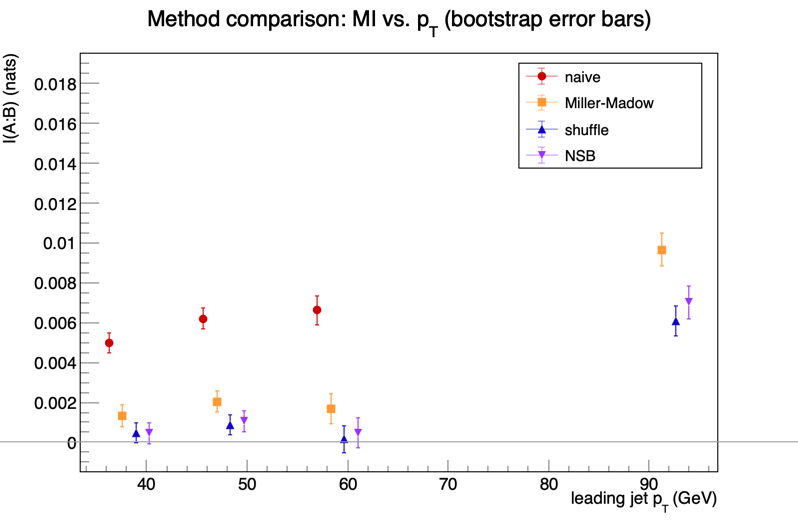
\includegraphics[width=0.48\textwidth]{figs/root_method_comparison_MI_vs_pt.png}
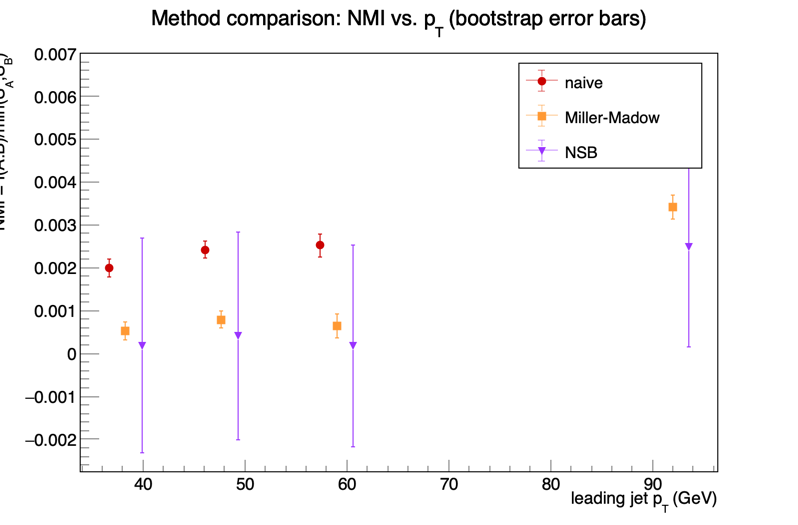
\includegraphics[width=0.48\textwidth]{figs/root_method_comparison_NMI_vs_pt_BUGGY.png}
\caption{The bug, illustrated: $I(A{:}B)$ method comparison (left,
unaffected) alongside the \emph{pre-fix} $\NMI$ method comparison (right)
from the same pipeline run. NSB's $\NMI$ error bars are visibly far wider,
relative to the central values, than $I$'s -- despite both being derived
from the same underlying quantities on the same events. This
discrepancy was the symptom that led to identifying the mixed-methodology
bug described in the text.}
\label{fig:root-nmi-bug}
\end{figure}

\begin{figure}[htb]
\centering
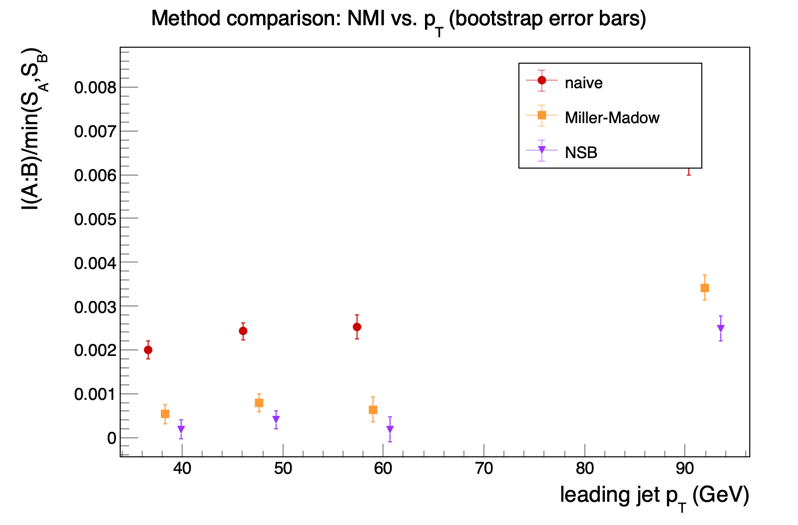
\includegraphics[width=0.48\textwidth]{figs/root_method_comparison_NMI_vs_pt_FIXED.png}
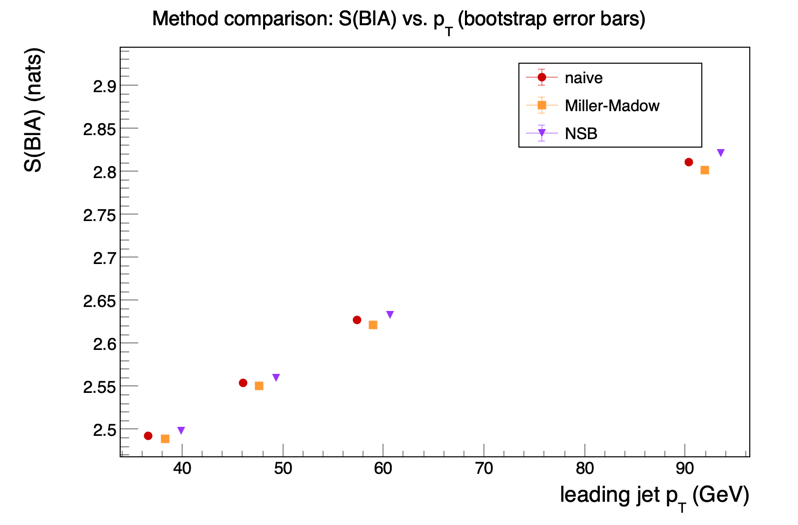
\includegraphics[width=0.48\textwidth]{figs/root_method_comparison_SBA_vs_pt.png}
\caption{Post-fix confirmation, same pipeline and dataset as
Fig.~\ref{fig:root-nmi-bug}: $\NMI$ method comparison (left) now shows
NSB error bars comparable in relative size to naive/Miller--Madow's, in
line with $I(A{:}B)$'s panel in Fig.~\ref{fig:root-nmi-bug} -- the
mixed-methodology discrepancy is gone. $\SBA$ method comparison (right,
never affected by this particular bug) shown alongside for reference,
confirming consistent bootstrap behavior across all three quantities.}
\label{fig:root-nmi-fixed}
\end{figure}

\paragraph{The general lesson.} When an uncertainty is obtained by
bootstrap resampling, every derived quantity built from the same
underlying estimate should be bootstrapped \emph{together, from the same
resamples} -- not by mixing bootstrap for some derived quantities and
analytic error propagation for others, even when both individually seem
reasonable. This also happens to be the more \emph{correct} choice
statistically, not merely the more consistent one: bootstrapping a ratio
directly captures the true correlation between numerator and denominator
(both estimated from the same event sample), whereas independence-
approximation error propagation assumes that correlation away and is
therefore both methodologically inconsistent \emph{and} typically
biased toward overly conservative (too large) uncertainties. This
pitfall generalizes beyond $\NMI$: any pipeline computing multiple
derived statistics from one bootstrap procedure should verify that
\emph{all} of them are actually using the same resamples, not just that
each individually looks plausible.

% =============================================================================
\section{Tier-2 closure test: calibrating estimator uncertainty on
realistic data}
\label{sec:closure}
% =============================================================================

The toy study (Secs.~\ref{sec:toymc}--\ref{sec:nsb}) validates
the estimator suite against a \emph{known} true MI, by construction. Real
PYTHIA~8 output, and eventually real STAR/ALICE data, has no such known
truth to validate against directly. This section describes a closure test
that closes that gap as far as is practically possible: calibrate a
synthetic model \emph{to resemble the real data}, use that model to
generate a pseudo-truth precise enough to treat as exact, and check
whether the estimator pipeline recovers it under closure -- i.e.\ under
exactly the statistical conditions (sample size, alphabet, correlation
strength) of the real measurement.

\subsection{Method}
\label{sec:closure-method}

\begin{enumerate}
\item \textbf{Calibrate.} Fit the toy study's Gamma-Poisson shared-latent
model (Sec.~\ref{sec:toymc}: $\Lambda\sim\mathrm{Gamma}(k,\theta)$,
$N_A|\Lambda\sim\mathrm{Poisson}(\Lambda)$,
$N_B|\Lambda\sim\mathrm{Poisson}(c\Lambda)$) to the \emph{real} data's
five leading moments -- $\langle N_A\rangle$, $\mathrm{Var}(N_A)$,
$\langle N_B\rangle$, $\mathrm{Var}(N_B)$, $\mathrm{Corr}(N_A,N_B)$ --
via least squares over $(k,\theta,c)$. This is a genuine, honest
constraint: a 3-parameter model cannot exactly match 5 targets in
general, and the achieved fit quality is reported explicitly rather than
assumed.
\item \textbf{Establish a pseudo-truth.} Draw a very large sample
(typically $10^6$--$5\times10^6$ events) from the \emph{fitted} model.
At this scale the naive estimator's own bias
($\mathcal{O}(1/N)$, Sec.~\ref{sec:bias}) is negligible, so $I,\SBA,\NMI$
computed on this sample are treated as numerically exact
($I_{\rm true},\SBA_{\rm true},\NMI_{\rm true}$) -- calibrated to
resemble the real measurement's shape and correlation strength, not an
arbitrary toy scenario.
\item \textbf{Closure.} Draw $N_{\rm repeats}$ independent fresh samples
from the fitted model, each at the real dataset's actual event count $N$
(and using the real analysis's alphabet), and run the full
naive/Miller--Madow/shuffle/NSB pipeline on each.
\item \textbf{Check bias and calibration.} For NSB specifically, form the
\emph{pull} for each repeat,
$z = (\hat X_{\rm NSB}-X_{\rm true})/\sigma_{\rm NSB}$
for $X\in\{I,\SBA,\NMI\}$, using that repeat's own bootstrap
$\sigma_{\rm NSB}$ (Sec.~\ref{sec:pitfall}). If the estimator is unbiased
and its uncertainty well-calibrated, the pull distribution across repeats
should be standard normal: mean $0$, standard deviation $1$, with
$\sim\!68\%$ of repeats within $\pm1\sigma$ and $\sim\!95\%$ within
$\pm2\sigma$.
\end{enumerate}
This is purely diagnostic throughout -- no bias or coverage correction is
applied to any reported number anywhere in this note; the closure test's
role is to establish \emph{whether} the raw bootstrap uncertainty can be
trusted at face value for a given $(N,\text{alphabet})$, not to patch it.

\subsection{Whole-sample results}
\label{sec:closure-results}

Applying this to the full $14$~TeV validation sample
(Fig.~\ref{fig:closure-I}, $I(A{:}B)$; Fig.~\ref{fig:closure-nmi}, $\NMI$)
gives two consistent findings:

\begin{itemize}
\item \textbf{A mean pull of approximately $-1$}: NSB systematically
under-\emph{estimates} $I(A{:}B)$ (and correspondingly $\NMI$) by
roughly one of its own reported bootstrap-$\sigma$'s, on average, at this
sample's statistics. This is a real, non-negligible bias, though modest
in scale.
\item \textbf{A pull standard deviation of approximately $1.5$--$1.7$}:
the \emph{actual} spread of $(\hat X-X_{\rm true})$ across independent
repeats is $50$--$70\%$ \emph{larger} than what the reported bootstrap
$\sigma$ claims. In other words, \texttt{NSB} $\pm$ \texttt{bootstrap
$\sigma$} under-covers -- the quoted error bars are too tight. Any
uncertainty quoted from the raw bootstrap $\sigma$ at this
$(N,\text{alphabet})$ therefore understates the true uncertainty by
roughly this same factor (e.g.\ a nominal $3\sigma$ separation between
two measurements would correspond to a true separation closer to
$3/1.7\approx1.8\sigma$).
\end{itemize}
The pull distributions in both figures are also visibly non-Gaussian:
skewed, with a heavier negative tail extending to several $\sigma$ beyond
what a standard normal would predict, rather than a uniformly-widened but
still-symmetric Gaussian. This matters practically: a single multiplicative
correction to $\sigma$ (calibrating only the second moment) would not
fully correct the shape of the tail, which is the part most relevant to
any strong claim of a difference between datasets or between data and a
model baseline. Any downstream use of these bootstrap uncertainties
should treat this as a known, quantified limitation rather than an
assumption to be taken on faith -- exactly the purpose of running this
closure test before, not after, a real measurement.

\begin{figure}[htb]
\centering
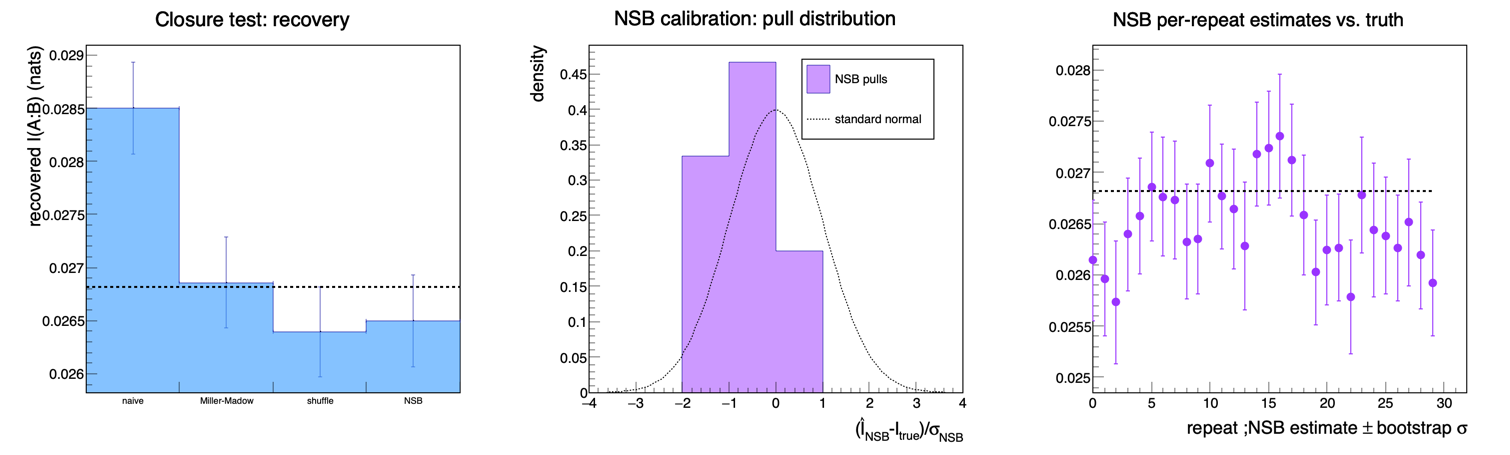
\includegraphics[width=\textwidth]{figs/closure_test_I.png}
\caption{Whole-sample closure test, $I(A{:}B)$: recovery across methods
(left), NSB pull distribution vs.\ standard normal (center), per-repeat
NSB estimates vs.\ the fitted-model pseudo-truth (right).}
\label{fig:closure-I}
\end{figure}

\begin{figure}[htb]
\centering
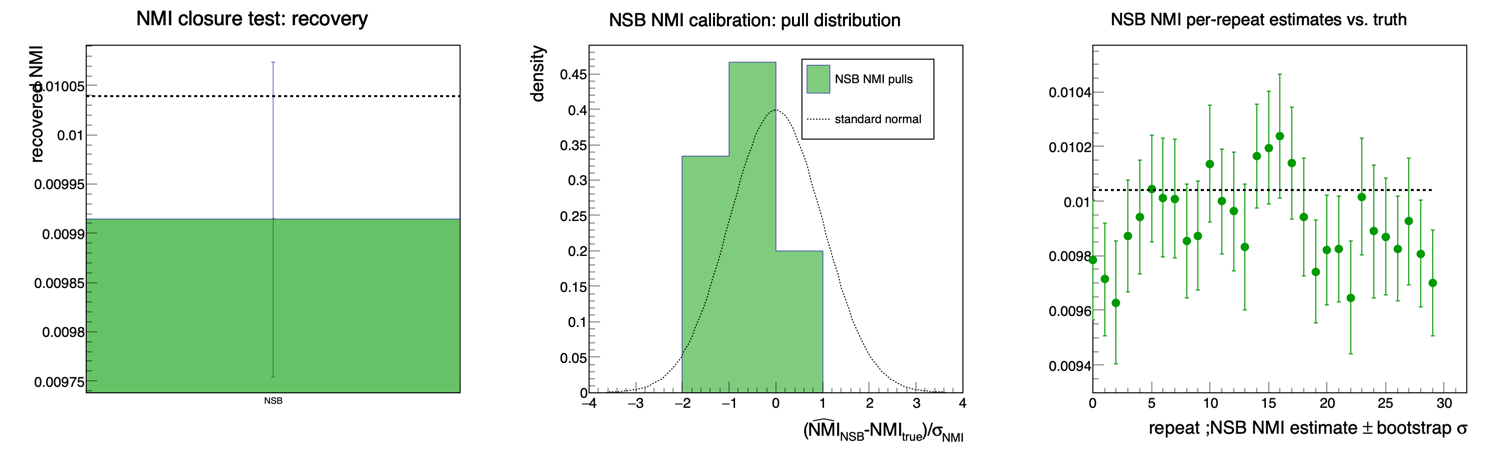
\includegraphics[width=\textwidth]{figs/closure_test_NMI.png}
\caption{Whole-sample closure test, $\NMI$: same three panels as
Fig.~\ref{fig:closure-I}, for the normalized observable.}
\label{fig:closure-nmi}
\end{figure}

\subsection{Extension to the conditional entropy directly}
\label{sec:closure-sba}

Sections~\ref{sec:closure-method}--\ref{sec:closure-results} were run
for $I(A{:}B)$ and $\NMI$; since $\SBA$ is the derived quantity whose
central value will be most directly interpreted physically -- and, per
Sec.~\ref{sec:nogo}, the one where residual estimator bias can
masquerade as spurious boundary-approaching structure -- a dedicated
closure test for $\SBA$ itself (mean pull, pull standard deviation, and
calibration fraction within $\pm1\sigma/\pm2\sigma$, identical procedure
to Sec.~\ref{sec:closure-method}) has been implemented and is not
inferred from $I$'s behavior via $\SBA=S_B-I(A{:}B)$ -- that inference
would carry $S_B$'s own separate estimation noise and is not a
substitute for a direct check. Numerical results for $\SBA$'s pull
distribution on this sample will be reported in a future revision of
this note.

\subsection{$p_T$-differential closure test}
\label{sec:closure-pt}

The results of Sec.~\ref{sec:closure-results} calibrate NSB's uncertainty
for a dataset shaped like the \emph{whole} sample -- but both the
underlying multiplicity/correlation structure and the per-bin event count
change with $p_T$ (Secs.~\ref{sec:pythia-ptdep},
\ref{sec:pythia}--\ref{sec:pythia-nmi}), so whole-sample calibration does
not automatically transfer to any individual $p_T$ bin, particularly the
highest-$p_T$, lowest-statistics bins where the correlation structure is
most interesting and least well-measured. A $p_T$-differential extension
of the closure test has been implemented: for each $p_T$ bin
independently, fit a bin-specific Gamma-Poisson model to that bin's own
events (not the whole-sample fit), generate a bin-specific pseudo-truth,
and run the closure procedure at that bin's actual event count --
directly answering ``is NSB's uncertainty trustworthy in \emph{this}
bin'' rather than assuming the whole-sample answer applies uniformly.

Figure~\ref{fig:closure-pt-summary} shows the result, in the same four
$p_T$ bins used throughout Sec.~\ref{sec:pythia-ptdep} ($p_T$ centers
$\approx38,48,59,92$~GeV). The pattern is notably different from, and in
one respect more encouraging than, the whole-sample result of
Sec.~\ref{sec:closure-results}:

\begin{itemize}
\item \textbf{Pull means} for $I(A{:}B)$ and $\NMI$ are small and
negative throughout ($\approx-0.12$ to $-0.17$ in the three lower-$p_T$
bins, shrinking to $\approx-0.04$ in the highest-$p_T$ bin) -- markedly
smaller in magnitude than the whole-sample $\approx-1$ found in
Sec.~\ref{sec:closure-results}. $\SBA$'s pull mean is somewhat larger at
low $p_T$ ($\approx-0.29$) but trends toward zero as $p_T$ increases,
reaching $\approx0$ in the highest-$p_T$ bin.
\item \textbf{Pull standard deviations} for $I(A{:}B)$ and $\NMI$ rise
from $\approx0.58$ (lowest-$p_T$ bin, i.e.\ \emph{over}-covering -- the
bootstrap $\sigma$ is if anything too conservative there) through
$\approx0.80$ and $\approx0.95$ to $\approx0.92$ in the highest-$p_T$
bin -- staying at or below $1$ throughout, in contrast to the
whole-sample $1.5$--$1.7$ under-covering. $\SBA$'s pull standard
deviation is close to $1$ in every bin ($\approx1.02,1.00,1.11,0.92$) --
the best-calibrated of the three quantities here, and encouragingly close
to ideal given $\SBA$ is the headline derived quantity of the eventual
measurement.
\end{itemize}

\begin{figure}[htb]
\centering
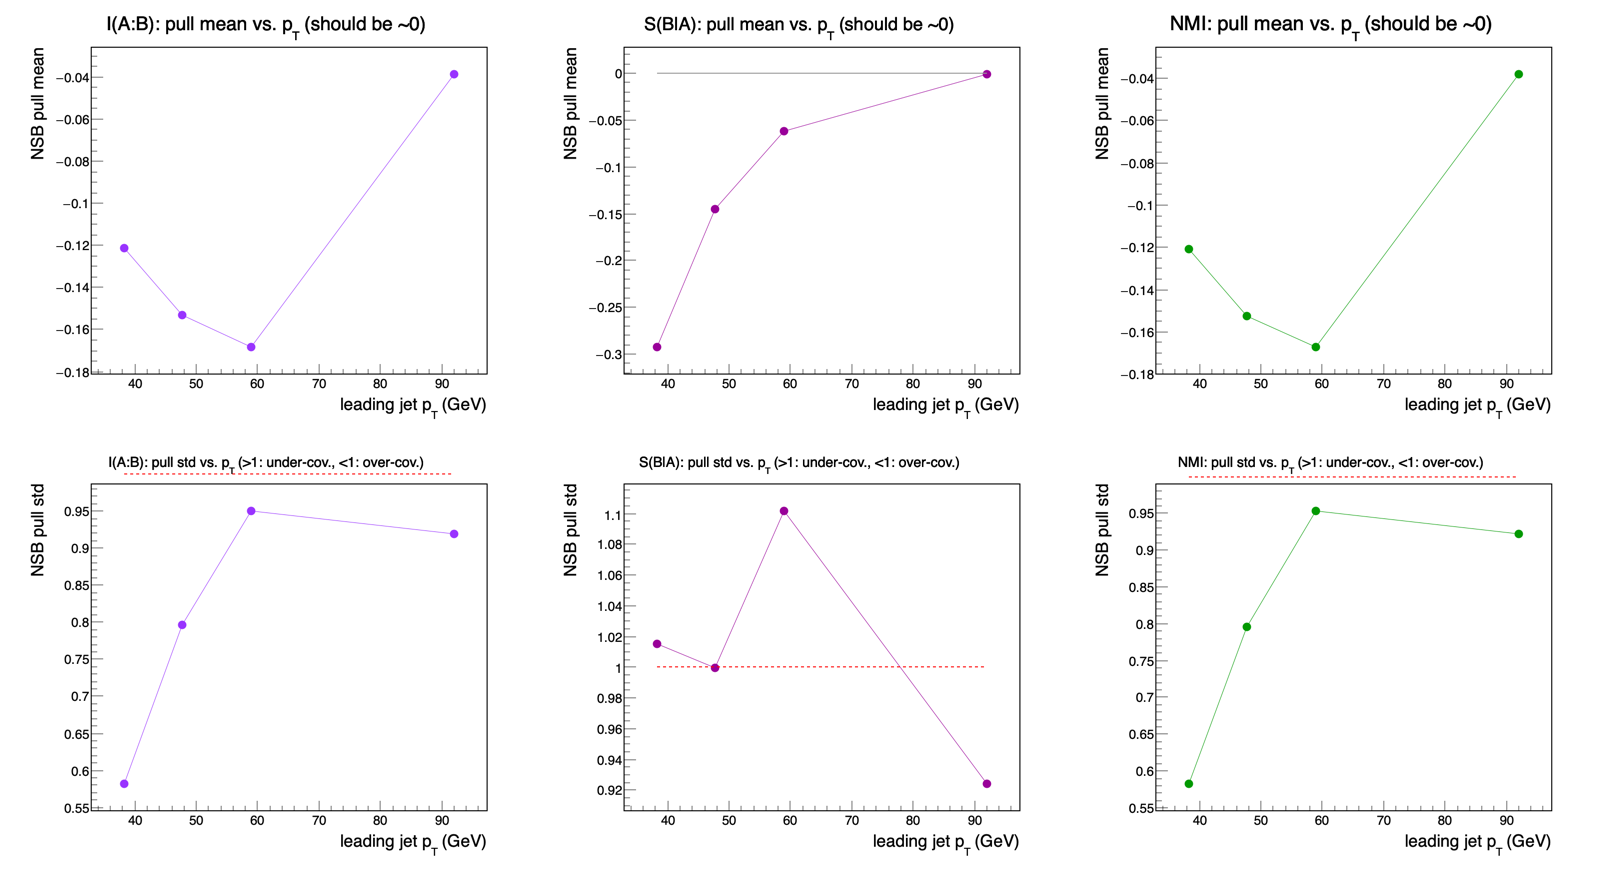
\includegraphics[width=\textwidth]{figs/closure_test_pt_summary.png}
\caption{$p_T$-differential closure test: NSB pull mean (top row) and
standard deviation (bottom row) vs.\ leading-jet $p_T$, for $I(A{:}B)$
(left), $\SBA$ (center), and $\NMI$ (right). Red dashed line marks
perfect calibration (pull std $=1$).}
\label{fig:closure-pt-summary}
\end{figure}

This bin-by-bin result being better-calibrated than the whole-sample one
is itself a meaningful, self-consistent finding, not merely a nicer
number: Sec.~\ref{sec:closure-pt}'s entire motivation was that the
whole-sample Gamma-Poisson fit has to compromise across a range of
$p_T$-dependent correlation structures at once (Sec.~\ref{sec:pythia-ptdep}),
whereas each bin-specific fit only has to describe its own,
comparatively homogeneous sub-population. A better-calibrated per-bin
result is exactly what that design difference predicts, and is evidence
the whole-sample closure test's miscalibration (Sec.~\ref{sec:closure-results})
is at least partly a model-fit-quality effect specific to forcing one
3-parameter model to span the full $p_T$ range, rather than a property of
NSB's bootstrap uncertainty in general. That said, this is a single
validation dataset at one set of statistics; whether this pattern holds
at STAR's actual $200$~GeV kinematics and statistics
(Sec.~\ref{sec:conclusions}) is not yet established and should not be
assumed.

Even with this more encouraging per-bin picture, no bin here reaches
pull std $=1$ exactly, and the lowest-$p_T$ bin's over-covering for
$I$/$\NMI$ ($\approx0.58$) is itself a $\sim\!40\%$ deviation from ideal
calibration, in the conservative direction. The practical recommendation
of Sec.~\ref{sec:closure-results} therefore still stands as the safe
default -- treat raw bootstrap $\sigma$ with caution and consult a
closure test at the actual bin/statistics in use -- with this section's
result showing that the correction, at least for this validation sample,
tends to be smaller and bidirectional per bin rather than a uniform
large under-coverage.

% =============================================================================
\section{Overall conclusions and next steps}
\label{sec:conclusions}
% =============================================================================

The toy Monte Carlo study (Secs.~\ref{sec:toymc}--\ref{sec:nsb})
establishes the estimator methodology and its failure modes under
controlled, known conditions. Section~\ref{sec:pythia} shows the same
pipeline, unmodified, correctly recovers physically-expected behavior
(NBD-like overdispersion, MLLA-consistent multiplicity growth with $p_T$,
the same finite-sample bias shape) on realistic QCD Monte-Carlo output
where no such structure was hand-built in -- a meaningful, if indirect,
validation that the pipeline is measuring real structure rather than an
artifact of the toy model's specific construction. An independent
ROOT/C++ re-implementation (Sec.~\ref{sec:pythia-nmi}) cross-validates the
Python results and adds $\NMI$, the scale-comparable normalized version
of the observable (Sec.~\ref{sec:observable}) needed to compare
measurements across $p_T$ bins, run periods, or collision energies on a
common, bounded scale.

That cross-validation also surfaced a genuine implementation bug
(Sec.~\ref{sec:pitfall}): a bootstrap-based derived quantity ($\NMI$)
picked up its uncertainty from an inconsistent, more conservative
analytic formula rather than the same resampling procedure used for
$I(A{:}B)$ and $\SBA$ in the same function. The fix, and more
importantly the general principle it illustrates -- every derived
quantity built from one bootstrap procedure must be resampled together,
not mixed with a separately-derived analytic error -- is recorded in
full since it is a pitfall relevant to any bootstrap-based entropy/MI
pipeline, not just this one.

Section~\ref{sec:closure} closes the gap the previous revision of this
note flagged as open: a closure test calibrated to resemble the real
PYTHIA~8 sample (Gamma-Poisson model fit to the real data's marginals and
correlation strength, huge reference sample for a pseudo-truth, repeated
closure at the real dataset's actual statistics) finds that NSB's
bootstrap uncertainty, at this sample's $(N,\text{alphabet})$, is
\textbf{under-covering by a factor of roughly $1.5$--$1.7$}, with a mean
bias of order $-1\sigma$ and a pull distribution that is skewed rather
than symmetrically widened. This is a quantitative, load-bearing result
for any future comparison of measured correlations across datasets or
against model baselines: a nominal $3\sigma$ difference computed from raw
bootstrap $\sigma$ at comparable statistics should be read as
$\sim\!1.8$--$2\sigma$ once this calibration factor is accounted for. Per
Sec.~\ref{sec:closure}, no correction has been baked into the pipeline
itself -- this factor is reported here as a measured property of the
estimator at these statistics, to be applied explicitly and cited
whenever an uncertainty is quoted, rather than silently folded into the
numbers.

The $p_T$-differential extension of the closure test (Sec.~\ref{sec:closure-pt})
is now complete for this validation sample, and adds an important
nuance: bin-by-bin, NSB's pull standard deviations sit much closer to
the ideal value of $1$ ($\approx0.58$--$0.95$ for $I(A{:}B)$ and $\NMI$;
$\approx0.92$--$1.11$ for $\SBA$) than the whole-sample result above,
consistent with each bin's own Gamma-Poisson fit describing a more
homogeneous sub-population than the one compromise fit spanning the
whole $p_T$ range has to. This suggests the whole-sample
under-coverage found in Sec.~\ref{sec:closure-results} is at least
partly a consequence of fitting one model across a range of
$p_T$-dependent structure, rather than an intrinsic property of NSB's
bootstrap procedure -- but this is one validation dataset at one set of
statistics, and the pattern should be re-checked, not assumed, at
STAR's actual kinematics. A dedicated whole-sample pull-distribution
check for $\SBA$ itself (Sec.~\ref{sec:closure-sba} -- distinct from its
per-bin counterpart just described, and still useful as the single most
directly load-bearing calibration number for the headline quantity)
remains to be run and will be reported in a future revision.

Remaining steps toward the actual STAR measurement: (i) repeat
Sec.~\ref{sec:pythia} at $\sqrt{s}=200$~GeV with STAR-appropriate jet
kinematics rather than the wide-dynamic-range $14$~TeV validation
kinematics used here; (ii) apply the detector-level acceptance and
tracking-efficiency model (already implemented in the generator, not yet
exercised in this note) and repeat the full analysis chain; (iii) rerun
the whole-sample and $p_T$-differential closure tests
(Secs.~\ref{sec:closure-results}--\ref{sec:closure-pt}) at the actual
statistics of (i)--(ii), obtaining calibration factors specific to the
real analysis rather than relying on the $14$~TeV validation sample's
factors as a proxy; (iv) once (i)--(iii) are complete, apply the
identical pipeline to real STAR data, with the closure-test calibration
factors from (iii) applied explicitly before unblinding, so that every
quoted $I(A{:}B)$, $\NMI$, and $\SBA$ value carries a defensible,
calibration-corrected uncertainty when compared against generator
baselines and the entanglement-ansatz expectations of
Sec.~\ref{sec:motivation}.

% =============================================================================
\begin{thebibliography}{99}

\bibitem{KL2017}
D.~E.~Kharzeev and E.~M.~Levin,
``Deep inelastic scattering as a probe of entanglement,''
Phys.\ Rev.\ D \textbf{95}, 114008 (2017),
arXiv:1702.03489.

\bibitem{PS2016}
R.~Peschanski and S.~Seki,
``Entanglement entropy of scattering particles,''
Phys.\ Lett.\ B \textbf{758}, 89 (2016),
arXiv:1602.00720.

\bibitem{TKU2020}
Z.~Tu, D.~E.~Kharzeev, and T.~Ullrich,
``Einstein--Podolsky--Rosen paradox and quantum entanglement at
subnucleonic scales,''
Phys.\ Rev.\ Lett.\ \textbf{124}, 062001 (2020),
arXiv:1904.11974.

\bibitem{H1_2021}
V.~Andreev \emph{et al.} [H1 Collaboration],
``Measurement of charged particle multiplicity distributions in DIS at
HERA and its implication to entanglement entropy of partons,''
Eur.\ Phys.\ J.\ C \textbf{81}, 212 (2021),
arXiv:2011.01812.

\bibitem{Datta2025}
J.~Datta, A.~Deshpande, D.~E.~Kharzeev, C.~J.~Na\"im, and Z.~Tu,
``Entanglement as a probe of hadronization,''
Phys.\ Rev.\ Lett.\ \textbf{134}, 111902 (2025),
arXiv:2410.22331.

\bibitem{CoverThomas}
T.~M.~Cover and J.~A.~Thomas,
\emph{Elements of Information Theory}, 2nd ed.\ (Wiley, 2006).

\bibitem{CerfAdami}
N.~J.~Cerf and C.~Adami,
``Negative entropy and information in quantum mechanics,''
Phys.\ Rev.\ Lett.\ \textbf{79}, 5194 (1997),
arXiv:quant-ph/9512022.

\bibitem{Kvalseth1987}
T.~O.~Kv\aa{}lseth,
``Entropy and correlation: Some comments,''
IEEE Trans.\ Syst.\ Man Cybern.\ \textbf{17}, 517 (1987).

\bibitem{OZ2001}
H.~Ollivier and W.~H.~Zurek,
``Quantum discord: A measure of the quantumness of correlations,''
Phys.\ Rev.\ Lett.\ \textbf{88}, 017901 (2001),
arXiv:quant-ph/0105072.

\bibitem{GPTV2022}
W.~Gong, G.~Parida, Z.~Tu, and R.~Venugopalan,
``Measurement of Bell-type inequalities and quantum entanglement from
$\Lambda$-hyperon spin correlations at high energy colliders,''
Phys.\ Rev.\ D \textbf{106}, L031501 (2022),
arXiv:2107.13007.

\bibitem{AfikDeNova2023}
Y.~Afik and J.~R.~Mu\~noz~de~Nova,
``Quantum discord and steering in top quarks at the LHC,''
Phys.\ Rev.\ Lett.\ \textbf{130}, 221801 (2023),
arXiv:2209.03969.

\bibitem{Miller1955}
G.~A.~Miller,
``Note on the bias of information estimates,''
in \emph{Information Theory in Psychology: Problems and Methods},
edited by H.~Quastler (Free Press, Glencoe, IL, 1955), pp.~95--100.

\bibitem{NSB2002}
I.~Nemenman, F.~Shafee, and W.~Bialek,
``Entropy and inference, revisited,''
in \emph{Advances in Neural Information Processing Systems 14} (MIT
Press, 2002),
arXiv:physics/0108025.

\bibitem{ALICE2024jets}
S.~Acharya \emph{et al.} [ALICE Collaboration],
``Multiplicity dependence of charged-particle intra-jet properties in
$pp$ collisions at $\sqrt{s}=13$~TeV,''
Eur.\ Phys.\ J.\ C \textbf{84} (2024),
arXiv:2311.13322.

\bibitem{ALICE2015fb}
J.~Adam \emph{et al.} [ALICE Collaboration],
``Forward-backward multiplicity correlations in $pp$ collisions at
$\sqrt{s}=0.9$, $2.76$ and $7$~TeV,''
JHEP \textbf{05}, 097 (2015),
arXiv:1502.00230.

\bibitem{DKMT1991}
Y.~L.~Dokshitzer, V.~A.~Khoze, A.~H.~Mueller, and S.~I.~Troyan,
\emph{Basics of Perturbative QCD} (Editions Fronti\`eres, Gif-sur-Yvette,
1991).

\end{thebibliography}

\end{document}
